% jxb: System Architecture and Internals
% Build: latexmk -pdf jxb.tex   (or: docker run --rm -v "$PWD":/doc jxb-tex:local latexmk -pdf jxb.tex)
\documentclass[11pt,a4paper]{article}

\usepackage[T1]{fontenc}
\usepackage[utf8]{inputenc}
\usepackage{lmodern}
\usepackage[scaled=0.95,varqu,varl]{inconsolata}
\usepackage{microtype}
\usepackage[a4paper,margin=2.3cm,headheight=14pt]{geometry}
\usepackage{amsmath,amssymb}
\usepackage{booktabs,tabularx,longtable,makecell,array}
\usepackage{graphicx}
\usepackage[table]{xcolor}
\usepackage{tikz}
\usetikzlibrary{positioning,arrows.meta,fit,backgrounds,shapes.geometric,shapes.misc,calc,decorations.pathreplacing}
\usepackage{pgfplots}
\pgfplotsset{compat=1.18}
\usepackage{listings}
\usepackage[most]{tcolorbox}
\usepackage{enumitem}
\usepackage{caption}
\usepackage{subcaption}
\usepackage{siunitx}
\usepackage{csquotes}
\usepackage{float}
\usepackage{fancyhdr}
\usepackage{algorithm}
\usepackage{algpseudocode}
\PassOptionsToPackage{hyphens,spaces,obeyspaces}{url}
\usepackage[colorlinks,linkcolor=jxbblue,urlcolor=jxbteal,citecolor=jxbteal]{hyperref}
\usepackage[nameinlink,capitalise]{cleveref}

\graphicspath{{../figures/}}

% ------------------------------------------------------------------------------------------------ colours
\definecolor{jxbblue}{HTML}{2F5D8A}
\definecolor{jxbteal}{HTML}{2A7F72}
\definecolor{jxborange}{HTML}{C7662B}
\definecolor{jxbred}{HTML}{B23A48}
\definecolor{jxbgray}{HTML}{5F6670}
\definecolor{jxblight}{HTML}{EEF3F8}
\definecolor{jxbgreen}{HTML}{E8F3EE}
\definecolor{jxbsand}{HTML}{FBF1E6}
\definecolor{codebg}{HTML}{F5F7F9}

% ------------------------------------------------------------------------------------------------ macros
\DeclareUrlCommand\code{\urlstyle{tt}}                 % inline code, breakable after / . _ - and at spaces
\newcommand{\codeb}[1]{\texttt{\detokenize{#1}}}      % inline code containing braces
\newcommand{\jxb}{\textsf{jxb}}
\newcommand{\finding}[1]{\textsf{\small F#1}}

\lstdefinelanguage{cmake}{
  morekeywords={set,list,if,endif,foreach,endforeach,string,file,message,find_program,APPEND,REMOVE_DUPLICATES,
    DEFINED,ENV,CACHE,NOT,IS_DIRECTORY,STRINGS,GLOB,REGEX,REPLACE,STRIP,IN,LISTS,ON},
  sensitive=true, morecomment=[l]{\#}, morestring=[b]"}
\lstdefinelanguage{toml}{morecomment=[l]{\#}, morestring=[b]", morestring=[b]', morekeywords={true,false}}
\lstdefinelanguage{docker}{morekeywords={FROM,RUN,ENV,ARG,USER,WORKDIR,CMD,SHELL}, morecomment=[l]{\#},
  morestring=[b]"}
\lstset{
  basicstyle=\ttfamily\footnotesize, backgroundcolor=\color{codebg}, frame=single, framerule=0pt,
  rulecolor=\color{codebg}, xleftmargin=5pt, xrightmargin=5pt, framexleftmargin=5pt, framexrightmargin=5pt,
  aboveskip=6pt, belowskip=6pt, breaklines=true, breakatwhitespace=false, columns=fullflexible, keepspaces=true,
  showstringspaces=false, upquote=true, keywordstyle=\color{jxbblue}\bfseries,
  commentstyle=\color{jxbgray}, stringstyle=\color{jxbteal}, tabsize=4,
  postbreak=\mbox{\textcolor{jxbgray}{$\hookrightarrow$}\space},
  captionpos=b, abovecaptionskip=4pt}

% ------------------------------------------------------------------------------------------------ boxes
\newtcolorbox{jxbnote}[1][Note]{colback=jxblight, colframe=jxbblue, boxrule=0.5pt, arc=2pt, left=6pt, right=6pt,
  top=3pt, bottom=3pt, fonttitle=\bfseries\small, coltitle=white, title=#1, fontupper=\small, before skip=8pt,
  after skip=8pt}
\newtcolorbox{jxbtip}[1][Why it matters]{colback=jxbgreen, colframe=jxbteal, boxrule=0.5pt, arc=2pt, left=6pt,
  right=6pt, top=3pt, bottom=3pt, fonttitle=\bfseries\small, coltitle=white, title=#1, fontupper=\small,
  before skip=8pt, after skip=8pt}
\newtcolorbox{jxbwarn}[1][Caution]{colback=jxbsand, colframe=jxborange, boxrule=0.5pt, arc=2pt, left=6pt,
  right=6pt, top=3pt, bottom=3pt, fonttitle=\bfseries\small, coltitle=white, title=#1, fontupper=\small,
  before skip=8pt, after skip=8pt}
\newtcolorbox{lesson}{colback=white, colframe=jxbteal, boxrule=0.4pt, leftrule=2.5pt, arc=0pt, left=6pt,
  right=6pt, top=2pt, bottom=2pt, fontupper=\small, before skip=6pt, after skip=8pt}

% ------------------------------------------------------------------------------------------------ TikZ styles
\tikzset{
  box/.style={draw=jxbblue!75, fill=white, rounded corners=2pt, align=center, font=\footnotesize, inner sep=3pt,
    minimum height=7.5mm, text width=#1},
  box/.default=26mm,
  hostbox/.style={box=#1, fill=jxblight},
  hostbox/.default=26mm,
  boardbox/.style={box=#1, draw=jxbteal!80, fill=jxbgreen},
  boardbox/.default=26mm,
  group/.style={draw=#1!70, fill=#1!5, rounded corners=4pt, inner sep=6pt},
  glabel/.style={font=\footnotesize\bfseries, text=#1, anchor=north west, inner sep=3pt},
  arr/.style={-{Stealth[length=2.2mm]}, semithick, draw=jxbgray},
  darr/.style={arr, dashed},
  lbl/.style={font=\scriptsize, text=jxbgray, fill=white, inner sep=1pt, align=center},
  pgroup/.style={draw=jxborange, dashed, rounded corners=3pt, inner sep=4pt},
  biarr/.style={semithick, draw=jxbgray, {Stealth[length=2.2mm]}-{Stealth[length=2.2mm]}},
}
\newcommand{\seqmsg}[4]{\draw[arr] (#1,#3) -- node[lbl,above=1pt]{#4} (#2,#3);}
\newcommand{\seqret}[4]{\draw[darr] (#1,#3) -- node[lbl,above=1pt]{#4} (#2,#3);}

% ------------------------------------------------------------------------------------------------ layout
\setlength{\parskip}{3pt}
\setlength{\emergencystretch}{2.5em}
\setlist{itemsep=1pt, topsep=3pt}
\pagestyle{fancy}
\fancyhf{}
\fancyhead[L]{\small\textcolor{jxbgray}{\jxb: System Architecture and Internals}}
\fancyhead[R]{\small\textcolor{jxbgray}{\nouppercase{\leftmark}}}
\fancyfoot[C]{\small\thepage}
\renewcommand{\headrulewidth}{0.3pt}
\renewcommand{\arraystretch}{1.15}
\captionsetup{font=small, labelfont=bf}

\hypersetup{pdftitle={jxb: System Architecture and Internals}, pdfsubject={Cross-development, deployment and
  observability for ROS 2 on NVIDIA Jetson Orin}}

\begin{document}

% ======================================================================================================== title
\begin{titlepage}
\centering
\vspace*{2.5cm}
{\Huge\bfseries\textcolor{jxbblue}{jxb}\par}
\vspace{0.4cm}
{\LARGE System Architecture and Internals\par}
\vspace{0.6cm}
{\large A reproducible cross-development, deployment and observability\\ environment for ROS~2 on NVIDIA Jetson Orin\par}
\vspace{1.6cm}
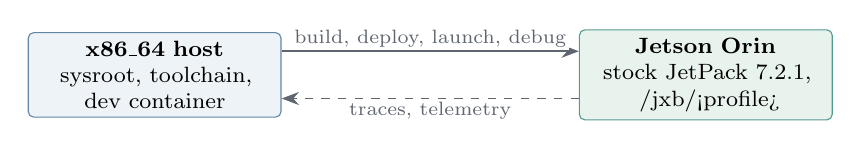
\begin{tikzpicture}[x=1cm,y=1cm]
  \node[hostbox=30mm] (h) at (0,0) {\textbf{x86\_64 host}\\sysroot, toolchain,\\dev container};
  \node[boardbox=30mm] (b) at (7,0) {\textbf{Jetson Orin}\\stock JetPack 7.2.1,\\\code{~/jxb/<profile>}};
  \draw[arr] ([yshift=3mm]h.east) -- node[lbl,above]{build, deploy, launch, debug} ([yshift=3mm]b.west);
  \draw[darr] ([yshift=-3mm]b.west) -- node[lbl,below]{traces, telemetry} ([yshift=-3mm]h.east);
\end{tikzpicture}
\vfill
{\large Technical documentation\par}
\vspace{0.2cm}
{Repository state after commit \code{bb3088a}, 2026-11-04\par}
\vspace{0.2cm}
{\small\url{https://github.com/sansrlian/jetson-xbuild}\par}
\vspace{1.5cm}
\end{titlepage}

% ======================================================================================================== abstract
\begin{abstract}
\noindent
Developing ROS~2 software with CUDA, TensorRT and ONNX Runtime for embedded NVIDIA Jetson Orin modules is commonly
done either directly on the board, which is slow and memory-bound, or in an emulated arm64 environment on a PC,
which is slower still and breaks for CUDA. Cross-compilation avoids both, but it is only correct if the build sees
exactly the libraries that the board will load at run time. This document describes \jxb, an environment that
(i)~constructs the target root file system (\emph{sysroot}) deterministically from the board's own package
repositories, without emulation and without access to a board; (ii)~compiles C++, CUDA and Python extension code
with an x86\_64 cross toolchain whose every component is pinned to the board's software release; (iii)~deploys,
runs, launches and debugs the result on unmodified, shared boards, either natively or in a GPU-enabled container
derived from the same sysroot; and (iv)~records and analyzes system behaviour with Nsight Systems, tegrastats,
per-process sampling, kernel tracing and inference benchmarks, emitting machine-readable summaries. The design is
inspired by the Renesas RZ/V2H RDK cross-build environment, whose structure it adopts; unlike the Jetson
workflow previously derived from it, the sysroot is constructed from a declarative profile instead of being copied
from a board. We describe the architecture
and each mechanism in depth, report measurements on an Orin Nano 8\,GB with JetPack~7.2.1 (for example, a
$3.2\times$ lower latency of the SAM detector model with a TensorRT fp16 engine than with ONNX Runtime's CUDA
execution provider, and the full SAM autonomy stack running at 2.8 CPU cores, 2.1\,GB and 8.4\,W), and discuss the
problems encountered during the implementation (62 recorded findings) and how they were resolved.
\end{abstract}

\vspace{0.5cm}
\noindent\textbf{How to read this document.} \Cref{sec:intro,sec:background} motivate the system and introduce the
concepts it relies on; \cref{sec:arch} gives the architecture overview; \cref{sec:sysroot,sec:toolchain,sec:deploy,sec:observe,sec:vscode}
are deep dives into the four subsystems and the editor integration; \cref{sec:eval} evaluates the system on the SAM
stack; \cref{sec:challenges,sec:process} discuss challenges and the implementation process. For day-to-day use, see
\code{docs/getting-started.md}; the engineering log \code{docs/findings.md} is cited as \finding{n}.

\newpage
\tableofcontents
\newpage

% ======================================================================================================== 1
\section{Introduction}\label{sec:intro}

\subsection{Motivation}
The system was built for the SAM project, an autonomous model vehicle whose ROS~2 stack (about 27 packages: camera
drivers, image processing with CV-CUDA, a YOLO object detector on ONNX Runtime, localization, an acados-based
trajectory planner and control) runs on NVIDIA Jetson Orin modules. Before \jxb, the team used a setup derived from
the Renesas RZ/V2H RDK~\cite{renesas-devguide}, which had five recurring problems (\cref{tab:problems}).

\begin{table}[H]
\centering\small
\caption{Problems of the previous workflow.}\label{tab:problems}
\begin{tabularx}{\textwidth}{@{}lXX@{}}
\toprule
& Problem & Effect \\
\midrule
P1 & The sysroot was synchronized (\code{rsync}) from a live board & not reproducible; drifts with every board; needs a prepared board before anything can be built \\
P2 & CUDA code was built in an emulated (QEMU) arm64 chroot & slow; \code{nvcc} and linking often failed, so CUDA packages were built on the board \\
P3 & Distribution mismatch & the stack targets ROS~2 Lyrical (Ubuntu 26.04), the board runs JetPack 7.2.1 (Ubuntu 24.04) \\
P4 & No multi-board view & no common deploy, trace collection or health view \\
P5 & CUDA minor-version drift & the desktop development image has CUDA 13.3, the board 13.2; TensorRT engines are version-bound \\
\bottomrule
\end{tabularx}
\end{table}

\subsection{Requirements}
From these problems and from the operating conditions (one shared lab board, several developers, later a fleet),
the following requirements were derived:
\begin{description}[leftmargin=1.1cm, labelindent=0pt, style=sameline, itemsep=0pt]
  \item[R1] \emph{Reproducibility.} The build environment is a function of a declarative profile, not of a board's history.
  \item[R2] \emph{Exact ABI match.} Every header and library used at build time is the version the board loads.
  \item[R3] \emph{No emulation for compilation.} C++, CUDA and Python extensions are compiled by native x86\_64 compilers.
  \item[R4] \emph{Boards stay stock.} No \code{apt} changes, no writes outside \code{~/jxb/}, no root; boards are shared.
  \item[R5] \emph{Several ROS~2 distributions} (Jazzy, Kilted, Lyrical) on the same stock board, switchable per command.
  \item[R6] \emph{One workflow, three front ends:} terminal, VS Code and, later, a GUI run the same operations.
  \item[R7] \emph{Observability with machine-readable results} (CPU, memory, GPU, power, scheduling, inference).
  \item[R8] \emph{Safety on shared hardware.} Measurements must not overlap; leftovers must not keep running.
\end{description}

\subsection{Contributions}
\begin{enumerate}
  \item A \textbf{sysroot builder} that resolves the arm64 package closure with a private \code{apt} instance against
        the board's repositories and reproduces the relevant side effects of maintainer scripts without executing
        them (\cref{sec:sysroot}).
  \item A \textbf{CMake/colcon cross toolchain} for C, C++, CUDA and Python extensions, including the corrections
        that CUDA 13.2, CMake and ROS~2 need for host builds (\cref{sec:toolchain}).
  \item A \textbf{board runtime model} that makes stock boards run other ROS distributions, either by shipping a
        relocatable ROS tree plus missing libraries (found by an \code{ldd} fix-point iteration) or by running a
        container image created from the sysroot itself (\cref{sec:deploy}).
  \item A \textbf{remote launch mode} in the style of the Renesas RDK, with process-group lifecycle management,
        monitoring and bag recording, and SSH-tunnelled remote debugging (\cref{sec:launch,sec:debug}).
  \item An \textbf{observability pipeline} that turns Nsight Systems databases, tegrastats logs, \code{/proc}
        samples and ftrace text into one \code{summary.json} per recording (\cref{sec:observe}).
  \item An \textbf{evaluation} on the SAM stack and a catalogue of findings, several of them upstream bugs
        (\cref{sec:eval,sec:challenges}).
\end{enumerate}

\subsection{Conventions}
\emph{Host} is the x86\_64 PC, \emph{board} the Jetson. Paths such as \code{~/jxb/<profile>} are board paths;
\code{sysroots/<profile>} is relative to the repository on the host. \code{<profile>} stands for a profile name such
as \code{jp721-kilted}. Code excerpts are taken from the repository and abridged where marked with \code{...}.

% ======================================================================================================== 2
\section{Background and concepts}\label{sec:background}
This section introduces the concepts the rest of the document relies on. Readers familiar with cross-compilation,
JetPack and colcon may skip to \cref{sec:arch}.

\subsection{Cross-compilation in a nutshell}
In GNU terminology, the \emph{build} machine runs the compiler and the \emph{host} machine runs the produced
program; embedded practice, and this document, call the PC \enquote{host} and the device \enquote{board} or
\enquote{target}. Producing correct binaries for another machine requires two ingredients:
\begin{enumerate}
  \item A \textbf{toolchain} that emits code for the target instruction set and ABI: here
        \code{aarch64-linux-gnu-gcc} (GCC~13, the default compiler of Ubuntu 24.04) and NVIDIA's \code{nvcc}.
  \item A \textbf{sysroot}: a directory that looks like the target's root file system for the purposes of compiling
        and linking. The compiler finds headers in \code{<sysroot>/usr/include}, the linker finds libraries in
        \code{<sysroot>/usr/lib/aarch64-linux-gnu}, and both treat \code{<sysroot>} as \code{/}.
\end{enumerate}
Linking against a shared library records information that the board's dynamic loader (\code{ld-linux-aarch64.so.1})
later relies on~\cite{elf-gabi}. These records explain most cross-build failures discussed in
\cref{sec:challenges} (\cref{tab:elf}).

\begin{table}[H]
\centering\small
\caption{ELF records that a cross build must get right.}\label{tab:elf}
\begin{tabularx}{\textwidth}{@{}lXX@{}}
\toprule
Record & Meaning & Typical cross-build failure \\
\midrule
\code{DT_NEEDED} & names of the libraries to load, normally their \code{SONAME} (e.g.\ \code{libcudart.so.13}) & an absolute host path is recorded when a library has no \code{SONAME} (\finding{44}) \\
\code{DT_RUNPATH} & search directories baked into the binary & host paths such as \code{/home/...} leak in \\
version needs & required symbol versions such as \code{GLIBC_2.38}, \code{GLIBCXX_3.4.32} & built against a newer glibc or libstdc++ than the board has \\
\code{PT_INTERP} & path of the dynamic loader & wrong loader for the target \\
ISA features & instruction-set extensions used by the code & \code{SIGILL} on a CPU without them (\finding{25}) \\
\bottomrule
\end{tabularx}
\end{table}

\begin{jxbnote}[Definition]
A sysroot is \emph{correct} for a board if, for every file the build reads, the sysroot's version is identical to the
version installed on the board. \jxb's central claim is that correctness can be established \emph{by construction}
(\cref{sec:sysroot}) instead of by copying.
\end{jxbnote}

\subsection{The Jetson Orin platform and JetPack 7.2.1}
The Orin modules combine Arm Cortex-A78AE cores with an NVIDIA Ampere GPU of compute capability~8.7
(\code{sm_87}) that shares the LPDDR5 memory with the CPU. All measurements in this document were taken on an
\textbf{Orin Nano 8\,GB} (6 cores, 7.3\,GB usable memory, 25\,W power mode, NVMe storage) running a
\textbf{PREEMPT\_RT} kernel (\code{6.8.12-rt-tegra}).

JetPack 7.2.1 is NVIDIA's software release for it~\cite{nvidia-jetson}: Jetson Linux (L4T) 39.2.1 on Ubuntu 24.04,
CUDA 13.2 (\code{cudart} 13.2.86), cuDNN 9.20, TensorRT 10.16.2, VPI 4.1 and an NVIDIA build of OpenCV 4.8
(\finding{1}). It is installed with \code{apt} from three NVIDIA repositories
(\code{common}, \code{som} and \code{ffmpeg} of release \code{r39.2} at \url{https://repo.download.nvidia.com/jetson/}), which an apt preference pins above Ubuntu's
packages with priority 600. Two platform details become important later:
\begin{itemize}
  \item CUDA 13 uses the unified Arm (\enquote{SBSA}) layout \code{targets/sbsa-linux} on Orin, not
        \code{aarch64-linux} as in JetPack~6 (\finding{2}).
  \item The CUDA driver is installed per GPU variant below \code{/opt/nvidia/l4t-gpu-libs/} (\code{nvgpu} for Orin, \code{openrm} for Thor); a boot
        service publishes the active one (\finding{26}). An extracted sysroot therefore has no \code{libcuda.so.1}
        until that step is replayed.
\end{itemize}

\subsection{ROS~2 builds: colcon, ament and code generators}
A ROS~2 workspace is built by \textbf{colcon}~\cite{colcon}, which builds each package (CMake or Python) in
dependency order and installs it into an \emph{install space}. Packages find each other through
\code{CMAKE_PREFIX_PATH}, \code{AMENT_PREFIX_PATH} and the ament resource index; at run time, generated
\code{setup.bash}/\code{local_setup.bash} scripts put the install space on \code{PATH}, \code{LD_LIBRARY_PATH} and
\code{PYTHONPATH}. The ROS installation itself (\code{/opt/ros/<distro>}) is the \emph{underlay}~\cite{ros2-docs}.

Cross-building ROS~2 is harder than cross-building a plain CMake project because \textbf{code generators run during
the build}: \code{rosidl} turns \code{.msg} files into C, C++ and Python sources, ament writes CMake configuration
files. These generators are Python programs that must run on the build machine, while the code they emit is
compiled for the target. \jxb{} therefore installs ROS~2 twice: on the host for the generators and in the sysroot
for the target libraries, both from the same distribution sync.

\subsection{The CUDA compilation model}
\code{nvcc}~\cite{nvcc} splits a \code{.cu} file into device code, which it compiles to GPU machine code (SASS) for
an architecture such as \code{sm_87} and optionally to PTX for just-in-time compilation, and host code, which it
passes to a host C++ compiler (\code{-ccbin}). Because \code{nvcc} itself is an x86\_64 program that needs only the
target's headers and libraries for the host part, it can cross-compile: with \code{-ccbin aarch64-linux-gnu-g++} and
\code{--target-directory sbsa-linux}, the device code is identical to a build on the board and the host code is
aarch64. This removes problem P2.

\subsection{The reference: the Renesas RZ/V2H RDK cross-build environment}\label{sec:renesas}
Renesas documents a cross-build setup for its RZ/V2H RDK that served as the model for \jxb's
structure~\cite{renesas-devguide,renesas-setup,renesas-vscode,renesas-faq}. Its development guide introduces the
concepts and limitations of cross-compiling, then walks through environment setup (a Docker image with an arm64
sysroot baked into \code{/opt/arm64_sysroot}), a usage guide (workspace layout, an arm64 chroot via QEMU for
\code{rosdep}, \code{cross-colcon-build}), a VS Code workspace with tasks for building, deployment and remote
debugging via \code{gdbserver}, a tutorial, known issues (for example, non-relocatable CMake paths inside the
sysroot) and an FAQ. Numbered procedures, notes and tips make it easy to follow. This document borrows that
structure: concepts first, then the architecture, then each workflow, with known issues and an FAQ at the end.

\jxb{} keeps the RDK's good ideas (one command per workflow, a long-lived build container, VS Code tasks that wrap
CLI commands, gdbserver debugging) and changes what did not scale for a Jetson fleet. The SAM team's earlier Jetson
workflow, derived from the RDK, synchronized its sysroot from live boards and built CUDA code in the emulated chroot
(P1, P2). \Cref{tab:renesas} compares the RDK image and that derived workflow with \jxb.

\begin{table}[H]
\centering\small
\caption{The RDK-based setup and \jxb.}\label{tab:renesas}
\begin{tabularx}{\textwidth}{@{}l>{\raggedright\arraybackslash}X>{\raggedright\arraybackslash}X@{}}
\toprule
Aspect & RDK-based setup & \jxb \\
\midrule
Sysroot origin & prebuilt, baked into the image (14.5\,GB image); for Jetson synchronized from boards & built from the board's apt repositories, per profile \\
Emulation & arm64 chroot (QEMU) for \code{rosdep}; in the Jetson workflow also for CUDA builds & none for compilation; QEMU only for optional smoke tests \\
CUDA & not part of the RDK (other SoC) & x86 \code{nvcc} of the board's exact version, \code{sm_87} \\
Distributions & one (Jazzy) & Jazzy, Kilted, Lyrical on 24.04, Lyrical on 26.04 \\
Boards & one configured target, password-based SSH (\code{sshpass}) & board inventory, SSH keys only, nothing installed on boards \\
Run-time modes & native & native or container, per command \\
Observability & not part of the cross-build guide & Nsight Systems, tegrastats, \code{/proc} sampling, ftrace, benchmarks \\
\bottomrule
\end{tabularx}
\end{table}

% ======================================================================================================== 3
\section{System architecture}\label{sec:arch}

\subsection{Overview}
\jxb{} consists of a host-side command-line interface and the artefacts it manages on the host and on the boards
(\cref{fig:arch}). The host holds four artefacts per profile: the \textbf{xbuild image} (host tools only,
$\approx$3.4\,GB), the \textbf{sysroot} (target files only, 16--19\,GB), the \textbf{dev container} that combines
both with the developer's workspace, and, for container mode, the \textbf{runtime image} (the sysroot without
build-only files). Boards receive only what a run needs, below \code{~/jxb/<profile>/}.

\begin{figure}[t]
\centering
\begin{tikzpicture}[x=1cm,y=1cm]
  % repositories
  \node[box=22mm] (u) at (1.3,6.45) {Ubuntu ports};
  \node[box=22mm] (n) at (1.3,5.55) {NVIDIA L4T r39.2};
  \node[box=22mm] (r) at (1.3,4.65) {ROS~2, Isaac ROS};
  % host, left column
  \node[hostbox] (sb) at (5.2,5.55) {sysroot builder\\\code{build_sysroot.py}};
  \node[hostbox] (sr) at (5.2,3.75) {\textbf{sysroot}\\\code{sysroots/<profile>}};
  \node[hostbox] (ri) at (5.2,1.3) {runtime image\\\code{jxb-rt:<profile>}};
  % host, right column
  \node[hostbox] (cfg) at (9.0,6.3) {profiles, \code{boards.toml}, \code{jxb.toml}};
  \node[hostbox] (cli) at (9.0,5.0) {\textbf{jxb CLI}\\Python, stdlib only};
  \node[hostbox] (img) at (9.0,3.7) {xbuild image\\GCC, nvcc, host ROS~2};
  \node[hostbox] (dev) at (9.0,2.4) {dev container\\workspace at host path};
  \node[hostbox] (tr) at (9.0,0.15) {\code{traces/<board>/...}\\\code{summary.json}, plots};
  % board
  \node[boardbox=27mm] (base) at (13.7,5.0) {\code{~/jxb/<profile>/}\\install, runtime, tools};
  \node[boardbox=27mm] (nat) at (13.7,3.3) {native mode\\bash + ROS};
  \node[boardbox=27mm] (con) at (13.7,1.3) {container mode\\Docker + CDI GPU};
  \node[boardbox=27mm] (rec) at (13.7,0.15) {recordings\\nsys, tegrastats, \dots};
  % groups
  \begin{scope}[on background layer]
    \node[group=jxbgray, fit={(u)(n)(r)(1.3,7.15)}] (gr) {};
    \node[group=jxbblue, fit={(sb)(sr)(ri)(cfg)(cli)(img)(dev)(tr)(3.9,7.15)}] (gh) {};
    \node[group=jxbteal, fit={(base)(nat)(con)(rec)(13.7,6.1)}] (gb) {};
  \end{scope}
  \node[glabel=jxbgray] at (gr.north west) {apt repositories};
  \node[glabel=jxbblue] at (gh.north west) {x86\_64 host};
  \node[glabel=jxbteal] at (gb.north west) {board, stock JetPack};
  % edges
  \draw[arr] (n.east) -- (sb.west);
  \draw[arr] (sb) -- node[lbl,right=2pt]{extract,\\emulate scripts} (sr);
  \draw[arr] (sr) -- node[lbl,right=2pt]{\code{docker import}} (ri);
  \draw[darr] (sr.east) -- node[lbl,left=1pt,pos=0.55]{bind mount, ro} (dev.west);
  \draw[arr] (cfg) -- (cli);
  \draw[arr] (cli.west) -- (sb.east);
  \draw[arr] (cli) -- (img);
  \draw[arr] (img) -- node[lbl,right=2pt]{\code{jxb up}} (dev);
  \draw[arr] (cli.east) -- node[lbl,above=1pt]{ssh, rsync\\keys only} (base.west);
  \draw[arr] (ri.east) -- node[lbl,below=1pt,pos=0.45]{\code{docker save | zstd}\\\code{| docker load}} (con.west);
  \draw[arr] (base) -- (nat);
  \draw[arr] (base.east) -- ++(0.35,0) |- (con.east);
  \draw[arr] (rec.west) -- node[lbl,above=1pt]{rsync} (tr.east);
\end{tikzpicture}
\caption{Components and data flows. Solid arrows produce or transfer data; the dashed arrow is a read-only bind
mount. The sysroot builder and the dev container both run in the xbuild image.}\label{fig:arch}
\end{figure}

\subsection{Components}
\Cref{tab:components} lists the components with their location and role. The CLI uses only the Python standard
library, so that it runs on any developer PC; everything that needs more (matplotlib, ROS, compilers) runs in the
dev container or on the board.

\begin{table}[t]
\centering\footnotesize
\caption{Components of \jxb.}\label{tab:components}
\begin{tabularx}{\textwidth}{@{}>{\raggedright\arraybackslash}p{2.5cm}>{\raggedright\arraybackslash}p{4.4cm}>{\raggedright\arraybackslash}p{1.9cm}>{\raggedright\arraybackslash}X@{}}
\toprule
Component & Location & Runs on & Role \\
\midrule
CLI & \path{jxb} & host & images, sysroot, container, build, boards, deploy, run, debug \\
launch mode & \path{toolchain/jxb_launch.py} & host$\to$board & deploy, \code{ros2 launch}, monitors, bags, helpers \\
tracing & \path{toolchain/jxb_trace.py} & host$\to$board & nsys, tegrastats, ftrace, benchmarks, analysis \\
plots & \path{toolchain/jxb_plot.py} & container & plots, \code{report.md}, comparisons \\
VS Code & \path{toolchain/jxb_vscode.py} & host & tasks and debug configurations \\
profile loader & \path{toolchain/jxb_profile.py} & host, container & TOML with \code{inherit} \\
xbuild image & \path{docker/xbuild.Dockerfile} & Docker & cross GCC, nvcc, host ROS~2, generators \\
sysroot builder & \path{sysroot/build_sysroot.py} & image & private apt, extraction, script emulation \\
package sets & \path{sysroot/sets/} & -- & what the sysroot contains \\
fixups & \path{sysroot/fixups.toml} & -- & patches for files that only break on the host \\
CMake toolchain & \path{toolchain/orin.toolchain.cmake} & container & C/C++/CUDA/Python cross settings \\
environment & \path{toolchain/env.sh}, \path{profile_env.py}, \path{ros-cross-env.sh} & container & variables derived from the sysroot's profile \\
build wrapper & \path{toolchain/bin/cross-colcon-build} & container & colcon with the toolchain, post-processing \\
binary checks & \path{jxb-elfcheck}, \path{jxb-fix-needed} & container & linkage verification, \code{DT_NEEDED} repair \\
dependency scan & \path{toolchain/bin/jxb-rosdeps} & image & rosdeps and launch-file dependencies \\
extras & \path{extras/} & container & ONNX Runtime GPU, acados, depthai \\
board tools & \path{tools/board/} & board & ftrace helper, benchmark, synthetic camera, bag$\to$CSV \\
tests & \path{tests/} & all & end-to-end check of a profile \\
\bottomrule
\end{tabularx}
\end{table}

\subsection{Profiles: the single source of truth}\label{sec:profiles}
A \textbf{profile} is a TOML file that pins everything that must match between the xbuild image, the sysroot and the
board: the JetPack/L4T version, CPU flags, CUDA version and architecture, the ROS distribution, the apt sources and
pins, the package sets and the extras (\cref{lst:profile}). Profiles inherit from one another; tables are merged
recursively, all other values are replaced (\cref{fig:profiles}):
\begin{lstlisting}[language=Python]
def _merge(base: dict, override: dict) -> dict:
    out = dict(base)
    for k, v in override.items():
        out[k] = _merge(out[k], v) if isinstance(v, dict) and isinstance(out.get(k), dict) else v
    return out
\end{lstlisting}

\begin{lstlisting}[language=toml, caption={Excerpt of the base profile \codeb{profiles/jp721-jazzy.toml}.}, label={lst:profile}]
[board]
jetpack = "7.2.1"
l4t = "39.2.1"
cpu_flags = "-mcpu=cortex-a78ae"
cuda_arch = "87"
gpu_variant = "nvgpu"              # JetPack 7.2 CUDA driver variant; Thor: openrm
ros_distro = "jazzy"

[image]
cuda_version = "13.2"
cuda_pkg_version = "13.2.86-1"     # must equal the board's cuda-cudart-13-2

[sysroot]
codename = "noble"
cuda_target = "sbsa-linux"
sources = [
    "deb [signed-by={ubuntu_key}] http://ports.ubuntu.com/ubuntu-ports noble main restricted universe multiverse",
    "deb [signed-by={nvidia_key}] https://repo.download.nvidia.com/jetson/common r39.2 main",
    ...
    "deb [signed-by={ros_key}] http://packages.ros.org/ros2/ubuntu noble main",
]
package_sets = ["base-dev", "runtime-base", "jetpack-7.2.1-dev", "l4t-driver", "ros-dev"]
extras = ["onnxruntime", "cvcuda", "acados"]
\end{lstlisting}

\begin{figure}[t]
\centering
\begin{tikzpicture}[x=1cm,y=1cm]
  \node[hostbox=46mm] (j) at (0,0) {\textbf{jp721-jazzy} (base)\\board, image, sysroot sources, keys, extras};
  \node[box=38mm] (k) at (-5.2,-2.0) {\textbf{jp721-kilted}\\\code{ros_distro = "kilted"}};
  \node[box=38mm] (i) at (0,-2.0) {\textbf{jp721-lyrical-isaac}\\Isaac ROS Buildfarm (noble),\\Isaac ROS 5, depthai};
  \node[box=38mm] (l) at (5.2,-2.0) {\textbf{jp721-lyrical}\\Ubuntu 26.04 sources,\\\code{ros_mode = "container"}};
  \foreach \c in {k,i,l} \draw[arr] (\c.north) -- node[lbl,pos=0.45]{inherit} (\c.north |- j.south);
\end{tikzpicture}
\caption{Profile inheritance: each child overrides only what differs from the base profile.}\label{fig:profiles}
\end{figure}

\begin{table}[H]
\centering\small
\caption{Profiles and how they run on a stock JetPack 7.2.1 board (which has ROS~2 Jazzy).}\label{tab:profiles}
\begin{tabularx}{\textwidth}{@{}llX@{}}
\toprule
Profile & ROS~2 / userland & On the board \\
\midrule
\code{jp721-jazzy} & Jazzy / Ubuntu 24.04 & the board's own ROS \\
\code{jp721-kilted} & Kilted / Ubuntu 24.04 & shipped to \code{~/jxb/jp721-kilted/runtime}, or container \\
\code{jp721-lyrical-isaac} & Lyrical (NVIDIA Buildfarm) + Isaac ROS 5.0 / Ubuntu 24.04 & shipped, or container \\
\code{jp721-lyrical} & Lyrical / Ubuntu 26.04 & container only (glibc 2.43) \\
\bottomrule
\end{tabularx}
\end{table}

The resolved profile is written into the sysroot (\code{.jxb/profile.json}) when the sysroot is built, and every
later step reads it from there. A sysroot and the settings it was built with can therefore never diverge
(\cref{sec:env}).

\subsection{Design principles}
\begin{enumerate}[label=\textbf{D\arabic*}]
  \item \textbf{Same repositories, same versions.} The sysroot is installed from the repositories, keys and pins the
        board itself uses, so its package versions are the board's by construction.
  \item \textbf{Extract, do not execute.} Packages are unpacked; the few maintainer-script effects that matter for
        compiling and linking are reproduced in Python. No QEMU, no root, no board.
  \item \textbf{Host paths everywhere.} Workspaces and the sysroot are mounted into the container at their host
        paths, so \code{compile_commands.json}, debug information and error messages are valid on the host and in
        the container alike.
  \item \textbf{The board is borrowed, not owned.} Everything \jxb{} deploys lives below \code{~/jxb/}; what the
        board lacks is shipped next to the deployment, never installed system-wide.
  \item \textbf{Every workflow is one non-interactive command} with a JSON form of its result (\code{--json},
        \code{summary.json}), so VS Code, scripts and a future GUI can drive the same code.
  \item \textbf{Fail loudly and early.} Missing keys, unresolved rosdeps, unbuilt packages, missing libraries and
        wrong ELF attributes stop the workflow with a message that says what to do.
\end{enumerate}

\subsection{Anatomy of a session}
\Cref{fig:session} shows what happens between typing \code{jxb build} and reading a performance report;
\cref{sec:sysroot,sec:toolchain,sec:deploy,sec:observe} explain each step.

\begin{figure}[t]
\centering
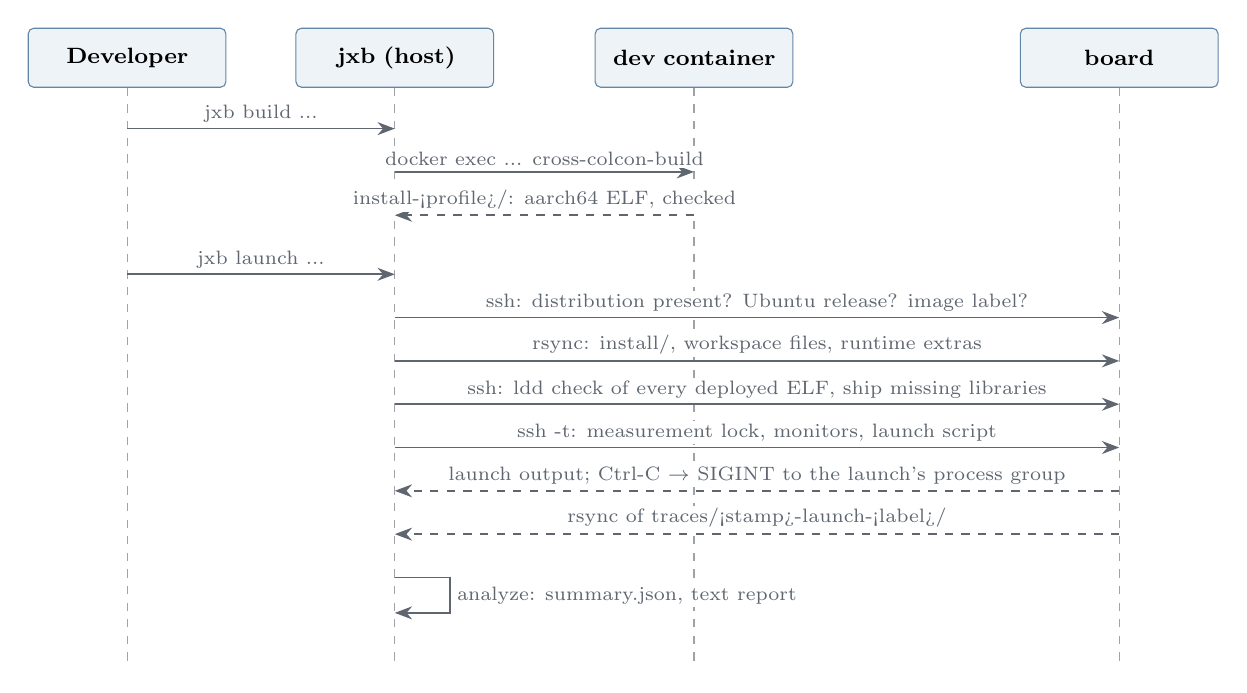
\begin{tikzpicture}[x=1cm,y=1cm]
  \foreach \x/\n/\t in {0/dv/Developer, 3.4/jh/jxb (host), 7.2/dc/dev container, 12.6/bd/board}{
    \node[box=23mm, fill=jxblight] (\n) at (\x,0) {\textbf{\t}};
    \draw[jxbgray!60, dashed] (\n.south) -- (\x,-7.7);
  }
  \seqmsg{0}{3.4}{-0.9}{\code{jxb build ...}}
  \seqmsg{3.4}{7.2}{-1.45}{\code{docker exec ... cross-colcon-build}}
  \seqret{7.2}{3.4}{-2.0}{\code{install-<profile>/}: aarch64 ELF, checked}
  \seqmsg{0}{3.4}{-2.75}{\code{jxb launch ...}}
  \seqmsg{3.4}{12.6}{-3.3}{ssh: distribution present? Ubuntu release? image label?}
  \seqmsg{3.4}{12.6}{-3.85}{rsync: \code{install/}, workspace files, runtime extras}
  \seqmsg{3.4}{12.6}{-4.4}{ssh: \code{ldd} check of every deployed ELF, ship missing libraries}
  \seqmsg{3.4}{12.6}{-4.95}{ssh -t: measurement lock, monitors, launch script}
  \seqret{12.6}{3.4}{-5.5}{launch output; Ctrl-C $\to$ SIGINT to the launch's process group}
  \seqret{12.6}{3.4}{-6.05}{rsync of \code{traces/<stamp>-launch-<label>/}}
  \draw[arr] (3.4,-6.6) -- ++(0.7,0) -- ++(0,-0.45) -- ++(-0.7,0);
  \node[lbl, right] at (4.15,-6.83) {analyze: \code{summary.json}, text report};
\end{tikzpicture}
\caption{A build, launch and analysis session.}\label{fig:session}
\end{figure}

% ======================================================================================================== 4
\section{Deep dive I: the sysroot builder}\label{sec:sysroot}

\subsection{Problem statement}
The sysroot must contain the headers, libraries, CMake and pkg-config files and Python modules of every package the
workspace builds against, \textbf{in the board's versions}, and in a form the host toolchain can use. Copying it from
a board (P1) violates R1 and R4: the result depends on the board's history, and it requires a board. Installing the
packages into an arm64 chroot with \code{apt} under QEMU is reproducible but slow, and it needs root, because
\code{dpkg} runs maintainer scripts.

The observation behind the builder is that \textbf{compiling and linking need only the files of a package and very
few side effects of its scripts}. Package \emph{resolution} can be done by \code{apt} running natively on the host if
\code{apt} is told that arm64 is its native architecture; \emph{extraction} is a \code{tar} operation; and the
relevant script effects can be enumerated (\cref{sec:scripts}). \Cref{fig:pipeline} gives the complete pipeline.

\begin{figure}[t]
\centering
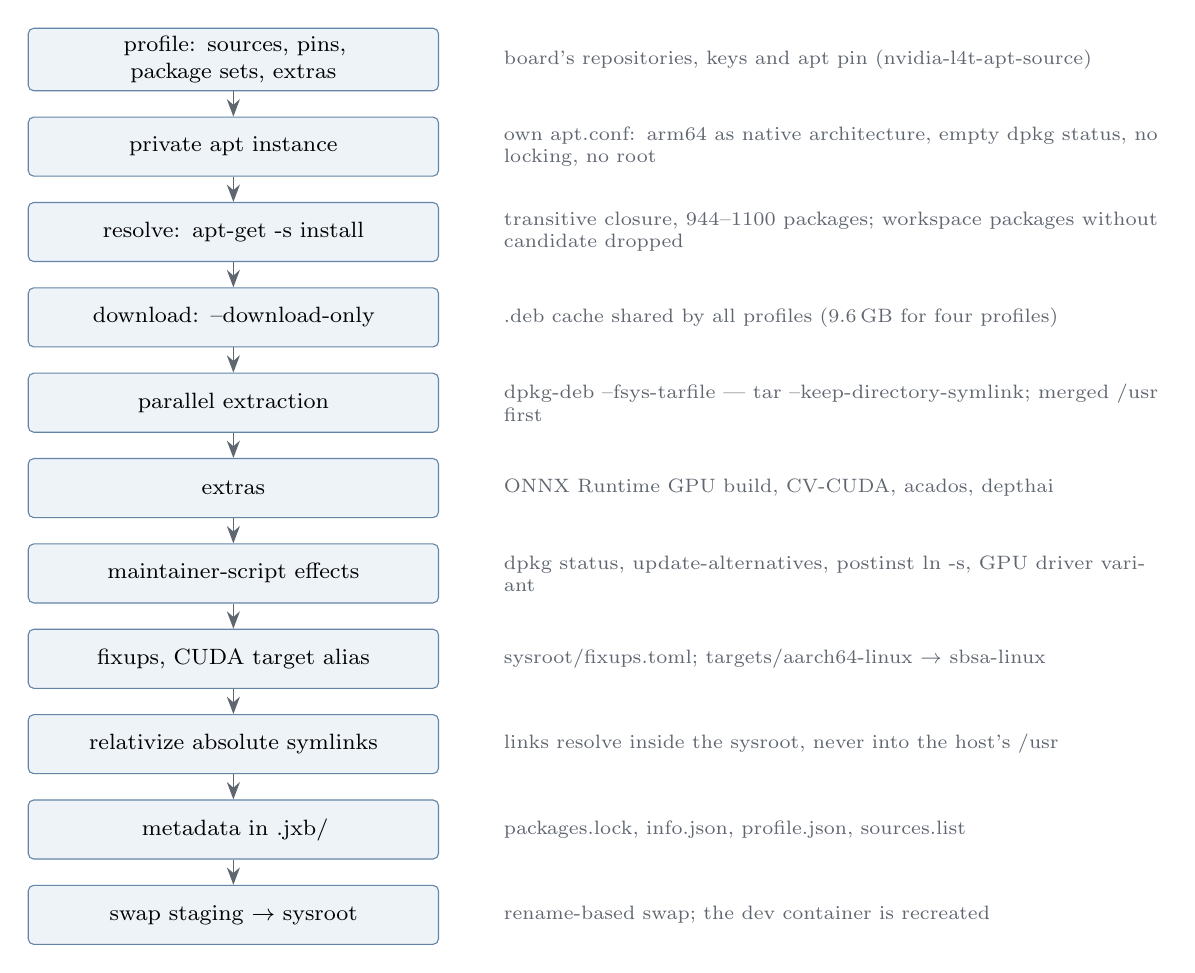
\begin{tikzpicture}[node distance=3.2mm and 7mm]
  \node[hostbox=50mm] (p) {profile: sources, pins, package sets, extras};
  \node[hostbox=50mm, below=of p] (a) {private apt instance};
  \node[hostbox=50mm, below=of a] (s) {resolve: \code{apt-get -s install}};
  \node[hostbox=50mm, below=of s] (d) {download: \code{--download-only}};
  \node[hostbox=50mm, below=of d] (x) {parallel extraction};
  \node[hostbox=50mm, below=of x] (e) {extras};
  \node[hostbox=50mm, below=of e] (m) {maintainer-script effects};
  \node[hostbox=50mm, below=of m] (f) {fixups, CUDA target alias};
  \node[hostbox=50mm, below=of f] (rl) {relativize absolute symlinks};
  \node[hostbox=50mm, below=of rl] (l) {metadata in \code{.jxb/}};
  \node[hostbox=50mm, below=of l] (w) {swap \code{staging} $\to$ sysroot};
  \foreach \u/\v in {p/a,a/s,s/d,d/x,x/e,e/m,m/f,f/rl,rl/l,l/w} \draw[arr] (\u) -- (\v);
  \tikzset{ann/.style={right=of #1, font=\scriptsize, text width=8.3cm, align=left, text=jxbgray}}
  \node[ann=p] {board's repositories, keys and apt pin (\code{nvidia-l4t-apt-source})};
  \node[ann=a] {own \code{apt.conf}: arm64 as native architecture, empty dpkg status, no locking, no root};
  \node[ann=s] {transitive closure, 944--1100 packages; workspace packages without candidate dropped};
  \node[ann=d] {\code{.deb} cache shared by all profiles (9.6\,GB for four profiles)};
  \node[ann=x] {\code{dpkg-deb --fsys-tarfile | tar --keep-directory-symlink}; merged \code{/usr} first};
  \node[ann=e] {ONNX Runtime GPU build, CV-CUDA, acados, depthai};
  \node[ann=m] {dpkg status, \code{update-alternatives}, \code{postinst ln -s}, GPU driver variant};
  \node[ann=f] {\code{sysroot/fixups.toml}; \code{targets/aarch64-linux} $\to$ \code{sbsa-linux}};
  \node[ann=rl] {links resolve inside the sysroot, never into the host's \code{/usr}};
  \node[ann=l] {\code{packages.lock}, \code{info.json}, \code{profile.json}, \code{sources.list}};
  \node[ann=w] {rename-based swap; the dev container is recreated};
\end{tikzpicture}
\caption{The sysroot build pipeline. No step executes target code.}\label{fig:pipeline}
\end{figure}

\subsection{A private apt instance}
\code{PrivateApt} creates a self-contained apt configuration in the profile's cache: its own \code{sources.list}
(the profile's \code{sources} with the downloaded keyrings substituted for \codeb{{nvidia_key}} and the like), its
own preferences (the board's pin), package lists, an archive cache and an \textbf{empty dpkg status file}. With
\code{APT_CONFIG} pointing at the file in \cref{lst:aptconf}, \code{apt-get} behaves as if it managed an empty
arm64 system.

\begin{lstlisting}[caption={Configuration of the private apt instance (generated).}, label={lst:aptconf}]
Dir "<cache>/apt/";
Dir::State::status "<cache>/apt/var/lib/dpkg/status";      // empty: nothing is installed
Dir::Cache::Archives "<deb-cache>/";                       // shared between profiles
APT::Architecture "arm64";
APT::Architectures { "arm64"; };
APT::Install-Recommends "false";
APT::Install-Suggests "false";
Debug::NoLocking "true";                                   // no root needed
\end{lstlisting}

Two details are easy to get wrong. First, apt's \code{signed-by} option decides the key format by file extension
(\code{.asc} for ASCII-armored keys, \code{.gpg} for binary keyrings), while the ROS key is a binary keyring served
under a neutral name; the builder therefore names downloaded keys by their content (\finding{16}). Second, the pin
must be exactly the board's: NVIDIA's packages win with priority 600, except that the profiles pin Ubuntu's
\code{libopencv-dev} at 700, because ROS \code{cv_bridge} links Ubuntu's OpenCV 4.6 and mixing it with NVIDIA's 4.8
made every \code{cv_bridge} node load two OpenCV versions (\finding{17}).

\begin{jxbtip}
The preference block is copied from \code{nvidia-l4t-apt-source}, the package that configures apt on a JetPack
board. This is what makes design principle D1 hold: apt applies identical inputs to identical candidate sets and
therefore selects identical versions.
\end{jxbtip}

\subsection{Resolving the closure}
The requested packages are the union of the profile's package sets (\code{sysroot/sets/*.txt}, with
\codeb{{ros_distro}} substituted) and the workspace set generated by \code{jxb-rosdeps} (\cref{sec:sets}).
Resolution uses apt's own solver in simulation mode, and the selection is parsed from its output:
\begin{lstlisting}[language=Python]
INST_RE = re.compile(r"^Inst (\S+) (?:\[\S+\] )?\((\S+) .*\[(\S+)\]\)")

def resolve(self, packages: list[str]) -> list[tuple[str, str, str]]:
    out = self.apt("-s", "install", *packages, capture=True)
    sel = [m.groups() for m in map(INST_RE.match, out.splitlines()) if m]   # (name, version, arch)
    ...
\end{lstlisting}
A line of the form \code{Inst libnvinfer10 (10.16.2.10-1+cuda13.2 <origin> [arm64])} yields name, version and
architecture. Because the dpkg status is empty, the simulation returns the \textbf{complete transitive closure}:
944 packages for Jazzy, 995 for Kilted, 1068 for Lyrical with Isaac ROS and 1100 for Lyrical on Ubuntu 26.04.
\code{apt-get install --download-only} then fetches exactly these files into the shared \code{.deb} cache; the first
profile downloads about 8\,GB.

Packages of a workspace set that no configured repository provides (for example \code{depthai} for Lyrical on Ubuntu
24.04) are removed with a warning before the resolution (\code{apt-cache policy} shows no candidate), so a single
missing optional dependency does not fail the whole sysroot.

\subsection{Extraction}
A \code{.deb} file is an \code{ar} archive with a \code{control.tar} and a \code{data.tar}. The builder streams the
data archive into the staging directory and keeps the control files for \cref{sec:scripts}:
\begin{lstlisting}[language=Python]
def extract_deb(deb: Path, dest: Path, scripts_dir: Path) -> str:
    data = subprocess.Popen(["dpkg-deb", "--fsys-tarfile", str(deb)], stdout=subprocess.PIPE)
    tar = subprocess.run(["tar", "-x", "-C", str(dest), "--keep-directory-symlink", "--no-same-owner",
                          "--warning=no-timestamp", "-f", "-"], stdin=data.stdout, ...)
    ...
    run(["dpkg-deb", "-e", str(deb), str(ctrl_dir)])        # control files: postinst, ...
    return (ctrl_dir / "control").read_text()
\end{lstlisting}
\code{--keep-directory-symlink} matters because Ubuntu uses a \textbf{merged \code{/usr}}: \code{/lib}, \code{/bin}
and \code{/sbin} are symbolic links into \code{/usr}. The builder creates these links first, and \code{tar} must
follow them instead of replacing them with directories; otherwise \code{/lib/aarch64-linux-gnu} and
\code{/usr/lib/aarch64-linux-gnu} would become two different directories. Extraction runs in a thread pool with one
job per CPU; a complete rebuild from the cache takes about one minute.

\subsection{Emulating maintainer scripts}\label{sec:scripts}
\code{dpkg} runs \code{preinst} and \code{postinst} scripts that may create files the build needs. Executing them is
exactly what \jxb{} avoids (they are arm64 programs or call them, and often need root). Instead, the builder
reproduces the four effects that matter for building and linking~\cite{debian-policy}:
\begin{enumerate}
  \item \textbf{The dpkg status database.} Some build tools ask dpkg what is installed. The builder writes every
        control paragraph with \code{Status: install ok installed} into \code{var/lib/dpkg/status}.
  \item \textbf{\code{update-alternatives} links.} Many \code{-dev} packages register alternatives (BLAS/LAPACK,
        \code{cpp}). The builder parses literal calls
        \code{update-alternatives --install LINK NAME PATH PRIO [--slave ...]} from all \code{postinst} scripts and
        creates the links of the winning candidate (\cref{alg:alternatives}).
  \item \textbf{Literal \code{ln -s} in \code{postinst}.} CV-CUDA and VPI create their CMake configuration links and
        \code{ld.so.conf.d} entries with plain \code{ln -s}, partly through shell variables (\finding{13}). The
        builder replays \code{ln -s SRC DEST} lines and expands variables that the script assigns literally
        (\code{VAR="..."}); a line with an unknown variable is skipped rather than guessed.
  \item \textbf{The GPU driver variant.} At boot, JetPack's \code{nv-load-gpu-libs.sh} publishes the active CUDA
        driver variant (\finding{26}). The builder writes the same \code{/etc/ld.so.conf.d/000-nvidia-gpu-libs.conf}
        and the \code{libcuda.so} links for the profile's \code{gpu_variant} (Orin: \code{nvgpu}).
\end{enumerate}
Finally, because CMake versions before~4 only look for \code{targets/aarch64-linux} when cross-compiling CUDA for
aarch64, the builder adds that name as an alias of \code{targets/sbsa-linux} (\finding{2}).

\begin{algorithm}[t]
\caption{Replaying \codeb{update-alternatives} (dpkg's automatic mode).}\label{alg:alternatives}
\begin{algorithmic}[1]
\State $\mathit{best} \gets \emptyset$ \Comment{group name $\mapsto$ (link, path, priority, slaves)}
\For{each \code{postinst} script $s$ of the extracted packages}
  \For{each literal call \code{--install} $(\ell, g, p, \pi, \mathit{slaves})$ in $s$ without shell variables}
    \If{$p$ exists in the sysroot \textbf{and} ($g \notin \mathit{best}$ \textbf{or} $\pi > \mathit{best}[g].\pi$)}
      \State $\mathit{best}[g] \gets (\ell, p, \pi, \mathit{slaves})$
    \EndIf
  \EndFor
\EndFor
\For{each $(g, (\ell, p, \pi, \mathit{slaves})) \in \mathit{best}$}
  \State create relative links $\ell \to$ \code{/etc/alternatives/}$g \to p$
  \State do the same for every slave whose path exists
\EndFor
\end{algorithmic}
\end{algorithm}

\begin{jxbwarn}[Limitation]
The selection reproduces dpkg's \emph{automatic} mode. A board can still differ if someone selected an alternative
manually: on the Nano, BLAS and LAPACK point to the reference implementations while the sysroot selects OpenBLAS
(\finding{43}). Both have the same soname, so programs run, but gdb shows wrong symbols for these two libraries.
\end{jxbwarn}

\subsection{Relative symbolic links}
Packages contain absolute symbolic links such as
\code{libfoo.so} $\to$ \path{/usr/lib/aarch64-linux-gnu/libfoo.so.1}. Inside the sysroot on
the host, such a link points into the \emph{host's} \code{/usr} and silently links host libraries. The builder
rewrites every absolute link target $t$ of a link in directory $d$ into
\begin{equation}
  t' = \operatorname{relpath}\bigl(\mathrm{root} \oplus t,\; d\bigr),
\end{equation}
where $\oplus$ joins the sysroot root and the board path. The links then resolve inside the sysroot on the host, and
they still resolve correctly when the tree is used as a root file system (the runtime image, \cref{sec:modes}).
Links created for alternatives are computed against the \emph{physical} parent directory, because \code{/lib/cpp}
physically lives in \code{usr/lib} once \code{lib} $\to$ \code{usr/lib}.

\subsection{Fixups}
A few sysroot files are correct on the board but break when used from the host. Declarative rules in
\code{sysroot/fixups.toml} patch them; each rule names the file, a search string, its replacement and the reason
(\cref{tab:fixups}).

\begin{table}[H]
\centering\small
\caption{Fixups applied to sysroot files.}\label{tab:fixups}
\begin{tabularx}{\textwidth}{@{}>{\raggedright\arraybackslash}p{4.6cm}X@{}}
\toprule
Rule & Why it is needed \\
\midrule
\path{rosidl_adapt_interfaces.cmake}: \path{file(STRINGS ... ENCODING UTF-8)} & without the encoding, CMake splits lines at non-ASCII bytes, so any workspace below a path such as \texttt{.../HochschuleM\"unchen/...} fails to generate interfaces (\finding{11}, a ROS~2 bug) \\
\code{acados_template}: return after the build if \code{JXB_CROSS_BUILD} is set & acados generates, compiles and then \code{dlopen()}s the solver; an aarch64 library cannot be loaded by the x86 build process, and the failed load deleted the freshly built library (\finding{20}) \\
CUB \code{device_transform.cuh}, \code{tuning_transform.cuh}: specialization inside its namespace & a CUDA 13.2 bug~\cite{cccl-8833}: GCC 13/14 reject the qualified class-head name that nvcc's front end re-emits; it breaks ONNX Runtime's CUDA EP, also natively (\finding{22}) \\
\bottomrule
\end{tabularx}
\end{table}

\subsection{Extras}
Some software is not available as a suitable apt package:
\begin{itemize}
  \item \textbf{ONNX Runtime 1.31 with CUDA and TensorRT execution providers for \code{sm_87}.} The released aarch64
        CUDA EP plugin contains code only for \code{sm_89/90a/120a/121a} and no PTX, so it cannot run on Orin
        (\finding{8}). \jxb{} cross-builds ONNX Runtime (\code{extras/onnxruntime/build.sh}) in a \enquote{lean}
        flavour that keeps the contrib operators (the TensorRT EP requires them) but drops the LLM-specific kernel
        families; a full build was estimated at about 7\,h on the 20-core workstation (\finding{24}). The sysroot
        uses the local build automatically when it exists, else the CPU release; the release's CMake configuration
        expects \code{lib64/} and \code{include/onnxruntime/}, which the builder adds as links (\finding{9}).
  \item \textbf{CV-CUDA 0.16} from its release packages (by URL), \textbf{acados 0.5.2} and \textbf{depthai 3.10}
        cross-built by \jxb{}; depthai through vcpkg with an overlay triplet that chainloads the \jxb{} toolchain
        (\finding{34}, \finding{40}).
\end{itemize}

\subsection{Package sets and workspace dependencies}\label{sec:sets}
The sysroot's content is declared in package sets (\cref{tab:sets}).
\begin{table}[H]
\centering\small
\caption{Package sets.}\label{tab:sets}
\begin{tabularx}{\textwidth}{@{}lX@{}}
\toprule
Set & Content \\
\midrule
\code{base-dev} & \code{build-essential} (libc and libstdc++ headers, CRT files), Python headers and numpy, Eigen, yaml-cpp, Boost, OpenSSL, zlib, protobuf, \dots \\
\code{runtime-base} & Ubuntu's \emph{Essential} packages (\code{bash}, \code{coreutils}, \code{findutils}, \code{grep}, \dots), which apt never pulls in as dependencies but a container needs (\finding{48}) \\
\code{jetpack-7.2.1-dev} & CUDA 13.2 libraries and the target headers \code{nvcc} needs (pinned), cuDNN, TensorRT, VPI, \dots \\
\code{l4t-driver} & \code{nvidia-l4t-core}, \code{nvidia-l4t-cuda}, the \code{nvgpu} CUDA driver \\
\code{ros-dev} & \code{ros-<distro>-ros-base}, generators, Cyclone DDS, \code{cv_bridge}, \code{image_transport}, messages, \code{tf2_ros}, \dots \\
\code{isaac-ros-5}, \code{depthai-deps} & optional: Isaac ROS 5.0; system dependencies of depthai \\
\bottomrule
\end{tabularx}
\end{table}

Workspace dependencies are collected by \code{jxb sysroot rosdeps -w WS}, which runs \code{jxb-rosdeps} in the
xbuild image. It resolves all \code{rosdep} keys of the workspace for the board's Ubuntu release and ROS
distribution, and it \textbf{also scans launch files} for the packages they start or include:
\begin{lstlisting}[language=Python]
LAUNCH_PKG = re.compile(r"""\b(?:package|pkg)\s*=\s*["']([A-Za-z][A-Za-z0-9_]*)["']"""
                        r"""|(?:get_package_share_directory|FindPackageShare)\(\s*["']([A-Za-z][A-Za-z0-9_]*)["']""")
\end{lstlisting}
The scan was added after the shipped Kilted runtime failed with \enquote{package 'topic\_tools' not found}: the SAM
launch files start \code{topic_tools}, \code{rplidar_ros}, \code{mavros} and \code{robot_state_publisher} and include
\code{foxglove_bridge}, but no \code{package.xml} declares them. On a developer PC with a full ROS installation this
goes unnoticed; on a board runtime made from declared dependencies it does not (\finding{52}, \finding{60}). GUI
tools and simulators are excluded. Keys that do not resolve are an error; for a distribution built for another
Ubuntu release (Lyrical on 24.04), keys are retried against the release it targets and accepted only if they map to
\code{ros-<distro>-*} packages (\finding{31}).

\subsection{Metadata and the swap}
The builder writes metadata into \code{<sysroot>/.jxb/} (\cref{tab:meta}). The sysroot is assembled in
\code{<name>.staging} and swapped in by renaming, so an interrupted build never leaves a half-written sysroot behind.
Because a running dev container still sees the old, now deleted directory through its bind mount,
\code{jxb sysroot build} recreates the container with the same workspaces (\finding{14}).

\begin{table}[H]
\centering\small
\caption{Sysroot metadata.}\label{tab:meta}
\begin{tabularx}{\textwidth}{@{}llX@{}}
\toprule
File & Content & Used by \\
\midrule
\code{packages.lock} & \code{name=version} of every package & \code{jxb board check} \\
\code{sources.list} & the exact apt sources & audit \\
\code{info.json} & build time, counts, alternatives, links, extras with SHA-256, fixups & runtime image label, \code{jxb sysroot info} \\
\code{profile.json} & the fully resolved profile & \code{env.sh}, \code{cross-colcon-build}, extras \\
\bottomrule
\end{tabularx}
\end{table}

\subsection{Properties}
\begin{itemize}
  \item \textbf{Determinism.} For fixed repository contents, the output is a function of the profile, and
        \code{packages.lock} documents it; \code{jxb board check} compares it with a board. Repositories advance over
        time: the Nano had \code{rclcpp} 28.1.21 from an earlier sync while the sysroot had 28.1.22, and the board's
        cuDNN was 9.25 while JetPack specifies 9.20 (\finding{35}). Such patch-level differences are ABI-compatible
        and reported as \code{DIFF}.
  \item \textbf{Cost.} About 8\,GB of downloads once, then about one minute per rebuild; 16--19\,GB per sysroot.
  \item \textbf{No privileges.} Neither root, nor a board, nor emulation is needed.
\end{itemize}

% ======================================================================================================== 5
\section{Deep dive II: the cross toolchain}\label{sec:toolchain}

\subsection{The xbuild image}
\code{docker/xbuild.Dockerfile} builds a host-tools-only image ($\approx$3.4\,GB) per profile on the Ubuntu release of
the board's userland (24.04, or 26.04 for \code{jp721-lyrical}). Its layers are:
\begin{enumerate}
  \item build tools and the distribution's \code{gcc-aarch64-linux-gnu}/\code{g++-aarch64-linux-gnu} (GCC~13 on 24.04),
        the default compiler of the board's Ubuntu release; \code{qemu-user} for optional smoke tests;
  \item ROS~2 on the host (\code{ros-<distro>-ros-base}, the rosidl generators, \code{ros-dev-tools});
  \item NVIDIA's \textbf{x86\_64 \code{nvcc} of exactly the board's version} (\code{cuda-nvcc-13-2=13.2.86-1}), held at
        that version;
  \item build-time generators the SAM stack needs on the host: \code{acados_template}, casadi 3.7.2 and the x86
        \code{t_renderer} (\finding{20}, \finding{21});
  \item a non-root user with the host's UID/GID, so files written into mounted workspaces keep their owner.
\end{enumerate}
The \jxb{} tree is \emph{not} copied into the image but bind-mounted at \code{/opt/jxb}, so changes to the toolchain
take effect without rebuilding the image. The CUDA layer contains two deliberate modifications:
\begin{lstlisting}[language=docker]
RUN ... && cd /usr/local/cuda-${CUDA_DASH/-/.} \
    && ln -sfn targets/${CUDA_TARGET}/include include && ln -sfn targets/${CUDA_TARGET}/lib lib64 \
    && sed -i "1i _TARGET_DIR_ = targets/${CUDA_TARGET}" bin/nvcc.profile
ENV NVCC_CCBIN=aarch64-linux-gnu-g++
\end{lstlisting}
CMake's \code{FindCUDAToolkit} probes \code{nvcc -v} without flags and then used the \emph{x86\_64} CUDA include
directory for C++-only targets (\finding{5}). Making the board's target directory \code{nvcc}'s default, and the
aarch64 compiler its default host compiler, turns this toolkit into one that \emph{only} targets the board: even a
plain \code{nvcc x.cu} produces aarch64 code. The \code{targets/sbsa-linux} directory of the image is replaced at run
time by the sysroot's copy (\cref{sec:devcontainer}), so device code is compiled against exactly the board's CUDA
headers and libraries.

\begin{jxbtip}
Configure tools so that their \emph{defaults} are correct. Build systems probe compilers in many ways, and not every
probe passes the flags a toolchain file sets.
\end{jxbtip}

\subsection{Deriving the environment}\label{sec:env}
Every board-specific value reaches the toolchain through environment variables, and all of them are derived from one
place, the profile copy inside the sysroot (\cref{lst:envsh}). \code{profile_env.py} maps the profile to
\code{JXB_PROFILE}, \code{ROS_DISTRO}, \code{JXB_CPU_FLAGS} (\code{-mcpu=cortex-a78ae}), \code{JXB_CUDA_ARCH}
(\code{87}), \code{JXB_CUDA_VERSION} (\code{13.2}), \code{JXB_CUDA_TARGET} (\code{sbsa-linux}),
\code{JXB_PYTHON_VERSION} and \code{JXB_QEMU_CPU}. The container only needs \code{ARM64_SYSROOT}; everything else
follows from it.

\begin{lstlisting}[language=bash, caption={\codeb{toolchain/env.sh}, sourced by every shell in the container.}, label={lst:envsh}]
if [ -n "${ARM64_SYSROOT:-}" ] && [ -f "${ARM64_SYSROOT}/.jxb/profile.json" ]; then
    while IFS= read -r _jxb_line; do
        _jxb_name=${_jxb_line#export }; _jxb_name=${_jxb_name%%=*}
        if [ -z "${!_jxb_name:-}" ]; then eval "${_jxb_line}"; fi     # variables already set win
    done < <(python3 "${JXB_HOME:-/opt/jxb}/toolchain/profile_env.py" "${ARM64_SYSROOT}/.jxb/profile.json")
    export JXB_TOOLCHAIN_FILE="${JXB_HOME:-/opt/jxb}/toolchain/orin.toolchain.cmake"
fi
\end{lstlisting}

\subsection{The CMake toolchain file}
\code{toolchain/orin.toolchain.cmake} is the core of the cross build~\cite{cmake-toolchains}. It refuses to run
without the environment above and then configures five areas.

\paragraph{Compilers and search roots.}
\begin{lstlisting}[language=cmake]
set(CMAKE_SYSTEM_NAME Linux)
set(CMAKE_SYSTEM_PROCESSOR aarch64)
set(CMAKE_SYSROOT "$ENV{ARM64_SYSROOT}")
set(CMAKE_C_COMPILER aarch64-linux-gnu-gcc)
set(CMAKE_CXX_COMPILER aarch64-linux-gnu-g++)
# Append, never overwrite: toolchain files are read several times, and wrappers that
# chainload this file (vcpkg) add their own roots after the first read.
list(APPEND CMAKE_FIND_ROOT_PATH "${JXB_SYSROOT}")
if(DEFINED ENV{JXB_WS_INSTALL})                  # packages of the same colcon workspace
  string(REPLACE ":" ";" _jxb_ws "$ENV{JXB_WS_INSTALL}")
  list(APPEND CMAKE_FIND_ROOT_PATH ${_jxb_ws})
endif()
set(CMAKE_FIND_PACKAGE_RESOLVE_SYMLINKS ON)
set(CMAKE_FIND_ROOT_PATH_MODE_PROGRAM NEVER)     # programs: host tools
set(CMAKE_FIND_ROOT_PATH_MODE_LIBRARY ONLY)      # libraries, headers, packages: target only
set(CMAKE_FIND_ROOT_PATH_MODE_INCLUDE ONLY)
set(CMAKE_FIND_ROOT_PATH_MODE_PACKAGE ONLY)
\end{lstlisting}
\code{CMAKE_FIND_ROOT_PATH} re-roots every search into the sysroot. Packages built earlier in the same colcon run are
installed \emph{outside} the sysroot, so the workspace's install space is added as a second root. Two subtle bugs
shaped this block: the first version used \code{set()}, which lost vcpkg's roots on the second read of the file
(\finding{33}); and in a merged-\code{/usr} sysroot, a CMake configuration found through the link
\code{lib} $\to$ \code{usr/lib} computed its install prefix as the sysroot root, which
\code{CMAKE_FIND_PACKAGE_RESOLVE_SYMLINKS} prevents (\finding{39}).

\paragraph{Linker paths.} The board's dynamic loader finds transitive dependencies through \code{/etc/ld.so.conf.d}
and \code{LD_LIBRARY_PATH}; the cross linker reads neither. The toolchain therefore collects the sysroot's
\code{ld.so.conf.d} entries plus the directories that are only on the board's \code{LD_LIBRARY_PATH} (ROS, ONNX
Runtime) and passes each as \code{-Wl,-rpath-link}. \code{--sysroot} is repeated in the linker flags because CMake
passes no sysroot flag when the host compiler links CUDA targets (\finding{6}).

\paragraph{pkg-config.} \code{PKG_CONFIG_LIBDIR} lists only the sysroot's \code{.pc} directories and
\code{PKG_CONFIG_SYSROOT_DIR} re-roots their paths; \code{PKG_CONFIG_PATH} is cleared so that no host \code{.pc} file
can leak in.

\paragraph{Python.} The host interpreter runs the generators, but headers, \code{libpython} and the extension suffix
must be the board's. Without overriding the SOABI, extension modules would be named
\code{*.cpython-312-x86_64-linux-gnu.so} and would not import on the board:
\begin{lstlisting}[language=cmake]
foreach(_jxb_p Python3 Python)
  set(${_jxb_p}_EXECUTABLE /usr/bin/python3 CACHE FILEPATH "Host Python for code generators")
  set(${_jxb_p}_INCLUDE_DIR "${JXB_SYSROOT}/usr/include/python${_jxb_py}" CACHE PATH "")
  set(${_jxb_p}_LIBRARY "${JXB_SYSROOT}/usr/lib/aarch64-linux-gnu/libpython${_jxb_py}.so" CACHE FILEPATH "")
  set(${_jxb_p}_SOABI "cpython-${_jxb_pynodot}-aarch64-linux-gnu" CACHE STRING "")
endforeach()
set(PYTHON_MODULE_EXTENSION ".cpython-${_jxb_pynodot}-aarch64-linux-gnu.so" CACHE STRING "")  # pybind11
\end{lstlisting}

\paragraph{CUDA.}
\begin{lstlisting}[language=cmake]
set(CMAKE_CUDA_COMPILER "/usr/local/cuda-$ENV{JXB_CUDA_VERSION}/bin/nvcc")
set(CMAKE_CUDA_HOST_COMPILER aarch64-linux-gnu-g++)
if(NOT DEFINED CMAKE_CUDA_ARCHITECTURES)
  set(CMAKE_CUDA_ARCHITECTURES "$ENV{JXB_CUDA_ARCH}")                 # 87
endif()
set(CMAKE_CUDA_FLAGS_INIT
  "--target-directory $ENV{JXB_CUDA_TARGET} -Xcompiler=--sysroot=${JXB_SYSROOT},${_jxb_cpu_xc}")
set(ENV{CUDA_TOOLKIT_ROOT} "${JXB_CUDA_ROOT}")                       # legacy FindCUDA (F31)
\end{lstlisting}
The last line exists because the legacy \code{FindCUDA} module, still used by \code{isaac_ros_common}, takes the
cross target directory only from an environment variable (\finding{31}).

\subsection{What runs where}
\Cref{tab:where} lists which machine each step of a build is for; this distinction is the key to reasoning about any
cross-build error.

\begin{table}[H]
\centering\small
\caption{Where the steps of a cross build run and what they produce.}\label{tab:where}
\begin{tabularx}{\textwidth}{@{}>{\raggedright\arraybackslash}p{3.3cm}>{\raggedright\arraybackslash}p{3.9cm}>{\raggedright\arraybackslash}X>{\raggedright\arraybackslash}p{2.2cm}@{}}
\toprule
Step & Program runs on & Reads & Output for \\
\midrule
rosidl / ament generators & host (x86 Python, host ROS) & \code{.msg} files, templates & source code \\
C/C++ compilation & host (\code{aarch64-linux-gnu-g++}) & sysroot headers & board \\
CUDA device code & host (x86 \code{nvcc}) & sysroot \code{targets/sbsa-linux} & board GPU (\code{sm_87}) \\
CUDA host code & host (aarch64 GCC via \code{-ccbin}) & sysroot headers & board \\
linking & host (\code{aarch64-linux-gnu-ld}) & sysroot libraries, \code{-rpath-link} & board \\
acados solver generation & host (casadi, x86 \code{t_renderer}) & board headers & C code for the board \\
TensorRT engine build & \textbf{board} & ONNX model & board (device- and version-specific) \\
\bottomrule
\end{tabularx}
\end{table}

\subsection{\texorpdfstring{\codeb{cross-colcon-build}}{cross-colcon-build}}
The wrapper that \code{jxb build} runs in the container
\begin{enumerate}
  \item sources \code{env.sh} and refuses to run without a \jxb{} sysroot;
  \item partitions its arguments into colcon and CMake arguments (CMake's own long options such as \code{--fresh}
        stay CMake's) and forbids overriding \code{CMAKE_TOOLCHAIN_FILE};
  \item adds defaults unless given: \code{CMAKE_BUILD_TYPE=Release}, \code{BUILD_TESTING=OFF},
        \code{CMAKE_EXPORT_COMPILE_COMMANDS=ON};
  \item uses per-profile trees \code{build-<profile>/} and \code{install-<profile>/}, so one workspace can be built for
        several distributions side by side;
  \item sources \code{ros-cross-env.sh}: host ROS Python modules first and the sysroot's (pure Python) as fallback,
        \code{AMENT_PREFIX_PATH} and \code{CMAKE_PREFIX_PATH} at the sysroot's \code{/opt/ros/<distro>},
        \code{CC}/\code{CXX} set to the board compiler for build steps that compile without CMake (acados' generated
        Makefiles), and \code{JXB_CROSS_BUILD=1};
  \item after the build, rewrites build-time paths and repairs ELF files (\cref{lst:post}).
\end{enumerate}
\begin{lstlisting}[language=bash, caption={Post-processing of the install space in \codeb{cross-colcon-build}.}, label={lst:post}]
# colcon's setup scripts and ament's parent_prefix_path index record the build-time underlay, i.e. the
# sysroot's copy of /opt/ros/<distro>. On the board that is plain /opt/ros/<distro>.
{ find "${install_base}" -maxdepth 1 -type f -name 'setup.*'
  find "${install_base}" -type f -path '*/share/ament_index/resource_index/parent_prefix_path/*'
} | xargs -r sed -i "s#${ARM64_SYSROOT}/#/#g"
"$(dirname "$(realpath "$0")")/jxb-fix-needed" "${install_base}"
\end{lstlisting}

\subsection{The dev container}\label{sec:devcontainer}
\code{jxb up} creates a long-lived container \code{jxb-<profile>} from the xbuild image with the mounts of
\cref{tab:mounts}. The board paths exist because SAM's \code{object_detection_package} hard-codes
\code{/opt/onnxruntime}, a board path (\finding{10}). Mounting workspaces at their host paths means that the absolute
paths in \code{compile_commands.json} and in the DWARF debug information are valid on the host, so clangd and gdb
work there without path maps.

\begin{table}[H]
\centering\small
\caption{Mounts of the dev container.}\label{tab:mounts}
\begin{tabularx}{\textwidth}{@{}l>{\raggedright\arraybackslash}X>{\raggedright\arraybackslash}X l@{}}
\toprule
Mount & Source & Target & Mode \\
\midrule
\jxb{} tools & repository & \code{/opt/jxb} and its own path & ro \\
sysroot & \code{sysroots/<profile>} & same path & ro \\
CUDA target & \path{<sysroot>/usr/local/cuda-13.2/targets/sbsa-linux} & \path{/usr/local/cuda-13.2/targets/sbsa-linux}, \path{.../aarch64-linux} & ro \\
board paths & \path{<sysroot>/opt/onnxruntime}, \path{<sysroot>/opt/acados} & \path{/opt/onnxruntime}, \path{/opt/acados} & ro \\
workspaces & each workspace & \textbf{same path} & rw \\
ccache & volume \code{jxb-ccache-<profile>} & \code{~/.ccache} & rw \\
\bottomrule
\end{tabularx}
\end{table}

\subsection{Verifying binaries}\label{sec:elf}
Two tools inspect every cross-built ELF file.

\code{jxb-elfcheck} parses \code{readelf} output and checks for each file that the machine type is AArch64, the
interpreter is \code{/lib/ld-linux-aarch64.so.1}, no \code{RUNPATH}/\code{RPATH} entry contains a host path, every
\code{DT_NEEDED} entry resolves the way it will on the board (\code{RUNPATH}, the install tree's library
directories, the sysroot's linker paths), no \code{DT_NEEDED} entry is an absolute path, and every required symbol
version (\code{GLIBC_*}, \code{GLIBCXX_*}, \dots) is defined by the library it resolves to. The last check catches
objects compiled against the cross compiler's own libc or libstdc++ instead of the board's (Ubuntu's cross GCC
searches its own directories before the sysroot, \finding{7}).

\code{jxb-fix-needed} repairs a defect that the linker produces legitimately. A shared library \emph{without}
\code{SONAME} that is linked by its full path is recorded by that path, here
\path{<sysroot>/opt/ros/lyrical/lib/libtensor_rt_node.so} (Isaac ROS exports its node libraries this way,
\finding{44}). The fix exploits a property of the ELF dynamic string table: the file name is a \emph{suffix} of the
recorded path, and strings are NUL-terminated, so pointing the \code{DT_NEEDED} entry at the offset of the suffix
yields the file name without moving a single byte (\cref{fig:dynstr}):
\begin{equation}
  \mathrm{off}' = \mathrm{off} + \lvert\mathrm{path}\rvert - \lvert\operatorname{basename}(\mathrm{path})\rvert .
\end{equation}
The tool walks \code{PT_DYNAMIC}, translates virtual addresses to file offsets through the \code{PT_LOAD} segments,
rewrites the matching \code{DT_NEEDED} entries and the \code{vn_file} fields of \code{.gnu.version_r} that name the
same library (the loader matches version requirements against the name by which it loaded a library), and writes the
file in place. Neither \code{patchelf} nor any section resizing is needed.

\begin{figure}[H]
\centering
\begin{tikzpicture}[x=1cm,y=1cm, cell/.style={draw=jxbgray!60, minimum height=6mm, font=\ttfamily\scriptsize, inner sep=1pt}]
  \node[cell, fill=jxbsand, minimum width=7.2cm] (a) at (3.6,0) {/home/.../sysroots/.../opt/ros/lyrical/lib/};
  \node[cell, fill=jxbgreen, minimum width=4.6cm, anchor=west] (b) at (a.east) {libtensor\_rt\_node.so};
  \node[cell, minimum width=0.6cm, anchor=west] (c) at (b.east) {\textbackslash 0};
  \draw[arr, jxborange] (0.0,1.0) node[above, font=\scriptsize, text=jxborange]{old \code{DT_NEEDED} offset} -- (a.north west);
  \draw[arr, jxbteal] (b.north west) ++(0,0.9) node[above, font=\scriptsize, text=jxbteal]{new offset} -- (b.north west);
  \node[font=\scriptsize, text=jxbgray] at (6.2,-0.75) {\code{.dynstr}: one NUL-terminated string, unchanged};
\end{tikzpicture}
\caption{Rewriting an absolute \codeb{DT_NEEDED} entry by moving its string offset to the file-name suffix.}\label{fig:dynstr}
\end{figure}

\subsection{The test suite}
\code{jxb test} cross-builds and checks probe projects that cover every layer: CUDA with relocatable device code and
cuBLAS (\code{cuda_hello}), a TensorRT engine build and inference (\code{trt_smoke}), ONNX Runtime with the CPU, CUDA
and TensorRT EPs (\code{ort_smoke}, \code{ort_bench}), the ONNX library built from source (\code{onnx_lib}), a ROS~2
workspace with a custom interface and a CUDA, TensorRT and \code{cv_bridge} node (\code{ros_ws}) and, for Isaac
profiles, a node that uses Lyrical's \code{rosidl::Buffer} CUDA backend (\code{isaac_ws}). On the host the stage is
checked with \code{jxb-elfcheck}, the extension-suffix check and runs under \code{qemu-aarch64 -cpu cortex-a76}, the
closest QEMU model to the Cortex-A78AE (QEMU~10's default model raises \code{SIGILL} on such code, \finding{25}).
\code{jxb test --board B} copies the stage to \code{~/jxb/<profile>/tests} and runs it on the GPU. The parsers of the
trace analysis have their own unit tests.

\paragraph{Continuous integration.} Three GitHub Actions workflows (\code{.github/workflows/}) run what fits where:
\begin{itemize}
  \item \code{ci.yml}, on every push and pull request: shellcheck of every shell script at warning level, a syntax
        check of every Python file, the trace analysis tests, and dry runs of \code{launch}, \code{trace tegrastats}
        and \code{vscode init} for the native profiles, against a CI board entry that names its Ubuntu release, so
        no command needs to ask a board;
  \item \code{image.yml}: builds the xbuild image of every profile when \code{docker/} or \code{profiles/} change;
  \item \code{board.yml}, on demand on a self-hosted runner labelled \code{jxb}: image, sysroot and the probe tests,
        optionally on a board. A sysroot takes 16--19\,GB, more than GitHub's hosted runners have.
\end{itemize}

% ======================================================================================================== 6
\section{Deep dive III: deployment and the board runtime}\label{sec:deploy}

\subsection{The board model}
Boards are listed in \code{boards.toml} (local, not committed) with host, user, optional SSH port, deployment
directory and tool overrides. All SSH calls use keys only (\code{BatchMode=yes}; a failed login prints the
\code{ssh-copy-id} command), \code{ConnectTimeout=8} and \code{StrictHostKeyChecking=accept-new}. Everything \jxb{}
writes lives in one directory per profile (\cref{lst:layout}).

\begin{lstlisting}[caption={Layout of a board's \codeb{~/jxb/} directory.}, label={lst:layout}]
~/jxb/
|-- .measure.lock, .measure.lock.info    measurement lock (flock) and its current holder
|-- trt_cache/                           TensorRT EP engine cache of the benchmarks
`-- <profile>/                           everything deployed for this profile; deletable at any time
    |-- <ws>/                            a deployed workspace (exported as WORKSPACE_ROOT)
    |   |-- install/                     install-<profile>/ of the host
    |   |-- launch/  assets/             workspace files
    |   `-- src/<pkg>/{launch,config,params,urdf}/
    |-- runtime/
    |   |-- opt/ros/<distro>/            shipped ROS distribution (only if the board lacks it)
    |   |-- opt/onnxruntime/ opt/acados/ runtime extras ([deploy] runtime)
    |   |-- pydist/                      Python modules the board's Python lacks
    |   `-- syslibs/                     shared libraries the board lacks
    |-- tools/                           board helpers (synthetic camera, bag to CSV, ftrace, benchmark)
    |-- tests/  bench/                   test stage; benchmark binaries, models and engines
    `-- traces/                          recordings in progress (fetched to the host, then removed)
\end{lstlisting}

\subsection{Deploying a workspace}
\code{deploy_workspace} performs, in order:
\begin{enumerate}
  \item \textbf{Board preparation}: in container mode, the runtime image is made available on the board; natively, the
        ROS distribution is shipped if the board lacks it (\cref{sec:ship}).
  \item \textbf{Incomplete packages.} A package that failed to build still leaves an install directory, because colcon
        writes \code{share/<pkg>/package.dsv} before building; its hooks name \code{local_setup.*} files that were
        never installed, and sourcing the workspace on the board then stops at that package (\finding{57}). Such
        packages are detected by checking that every \code{source;} hook in \code{package.dsv} exists; they are not
        deployed, and stale copies are removed.
  \item \textbf{The install space}, completely (\code{rsync --delete}) or only the requested \code{--packages} together
        with colcon's top-level setup files, using ordered rsync filter rules.
  \item \textbf{Workspace files} needed at run time but not installed: \code{launch/}, \code{assets/} and the
        \code{launch}, \code{config}, \code{params} and \code{urdf} folders of the packages. Files that are only
        \textbf{Git LFS pointers} (smaller than 1\,KiB and starting with \code{version https://git-lfs.github.com/spec/})
        are excluded, after a pointer once replaced the real model on the board (\finding{51}).
  \item \textbf{Runtime extras} (\code{[deploy] runtime}): \jxb's ONNX Runtime GPU build and acados go to
        \code{~/jxb/<profile>/runtime/opt/...}, never into the board's \code{/opt}.
  \item \textbf{Library closure check} (\cref{sec:ship}).
\end{enumerate}

\subsection{Making a stock board run another ROS distribution}\label{sec:ship}
The board runs Jazzy; Kilted and Lyrical must run without touching \code{apt} (R4, R5). Two observations make this
possible. First, ROS~2's setup scripts derive their prefix from their own location, so the sysroot's
\code{/opt/ros/<distro>} is \textbf{relocatable}: copied to \code{~/jxb/<profile>/runtime/opt/ros/<distro>} without
headers and static libraries (191\,MB for Kilted, 226\,MB for Lyrical with Isaac ROS), it runs from there
(\finding{44}). This requires the same Ubuntu release, which is checked against the board's
\code{VERSION_CODENAME}. Second, the remaining gaps can be found mechanically:
\begin{itemize}
  \item \textbf{Python modules.} Lyrical takes \code{osrf_pycommon} from the system package
        \code{python3-osrf-pycommon}, which the board has only inside \code{/opt/ros/jazzy}, so \code{ros2 launch}
        failed (\finding{61}). \code{ship_pydist} compares the sysroot's \code{dist-packages} with the modules the
        board's Python can import and ships the difference to \code{runtime/pydist}, appended to \code{PYTHONPATH}.
  \item \textbf{Shared libraries.} \code{ensure_board_libs} computes a fix point (\cref{alg:libs}): a script on the board
        prints \code{HAVE <file>} for every library below the deployed directories and \code{MISSING <soname>} for
        every library that \code{ldd} cannot resolve for any deployed ELF file; missing libraries are copied from the
        sysroot to \code{runtime/syslibs}, which is on \code{LD_LIBRARY_PATH}, and the check is repeated, because
        shipped libraries can have dependencies of their own.
\end{itemize}

\begin{algorithm}[t]
\caption{Library closure on the board (\codeb{ensure_board_libs}).}\label{alg:libs}
\begin{algorithmic}[1]
\Require deployed directories $D$; sysroot library directories $L$
\State $S \gets \emptyset$ \Comment{sonames shipped to \code{runtime/syslibs}}
\For{$k = 1, \dots, 5$}
  \State $(H, M) \gets$ run on the board: libraries present below $D$; sonames \code{ldd} cannot resolve
  \State $M \gets M \setminus (H \cup S)$
  \If{$M = \emptyset$} \Return \Comment{every deployed ELF file resolves}
  \EndIf
  \For{$m \in M$}
    \If{$\exists\, \ell \in L : \ell/m$ exists in the sysroot} copy it to the stage; $S \gets S \cup \{m\}$
    \Else\ \textbf{fail}: \enquote{missing on the board and not in the sysroot}
    \EndIf
  \EndFor
  \State rsync the stage to \code{runtime/syslibs}
\EndFor
\State \textbf{fail}: no fix point after five rounds
\end{algorithmic}
\end{algorithm}

In practice the board lacked no system library for Kilted or Lyrical on Ubuntu 24.04; the mechanism turns that into
a checked fact instead of an assumption.

\subsection{The board environment}
Every remote command is prefixed by a generated shell snippet whose order matters (\cref{lst:env}). The underlay is
sourced explicitly and the workspace through \code{local_setup.bash}, not \code{setup.bash}, because the underlay
path recorded at build time need not exist on the board. \jxb's ONNX Runtime comes first on \code{LD_LIBRARY_PATH}, so
it wins over the board's own CPU-only \code{/opt/onnxruntime} (\finding{38}). \code{set +u} is needed because ROS
setup scripts reference unset variables (\finding{37}).

\begin{lstlisting}[language=bash, caption={The environment prefix of a remote command (\codeb{board_env_script}; abridged, \codeb{P} = profile, \codeb{D} = distribution, \codeb{WS} = workspace).}, label={lst:env}]
set +u; export PYTHONPATH=${PYTHONPATH:+$PYTHONPATH:}~/jxb/P/runtime/pydist;               # native only
export JXB_ROS_SETUP=/opt/ros/D/setup.bash; [ -f $JXB_ROS_SETUP ] ||
    JXB_ROS_SETUP=~/jxb/P/runtime/opt/ros/D/setup.bash; source $JXB_ROS_SETUP &&           # 1. underlay
if [ -f ~/jxb/P/WS/install/local_setup.bash ]; then source ~/jxb/P/WS/install/local_setup.bash; fi &&  # 2.
export LD_LIBRARY_PATH=~/jxb/P/runtime/opt/onnxruntime/lib:~/jxb/P/runtime/opt/acados/lib:~/jxb/P/runtime/syslibs:$LD_LIBRARY_PATH &&
export WORKSPACE_ROOT=~/jxb/P/WS && export ROS_AUTOMATIC_DISCOVERY_RANGE=LOCALHOST && ...  # 3. jxb.toml env
\end{lstlisting}

\subsection{Native and container mode}\label{sec:modes}
\code{uses_container} decides where board commands run: an explicit \code{--mode native|container} (or \code{mode}
in \code{jxb.toml}) wins; otherwise a profile can force a mode (\code{[deploy] container}); otherwise the container
is used exactly when the profile's Ubuntu release differs from the board's. \code{board_exec} then wraps the script
(\cref{fig:modes}).

\begin{figure}[t]
\centering
\begin{tikzpicture}[x=1cm,y=1cm]
  \node[box=34mm] (s) at (0,0) {\code{board_env_script}\\+ command};
  \node[diamond, draw=jxbblue!75, aspect=2.2, inner sep=1pt, font=\footnotesize, align=center] (q) at (4.4,0) {container\\mode?};
  \node[boardbox=40mm] (n) at (9.6,1.3) {\code{bash -lc SCRIPT}};
  \node[boardbox=62mm, align=left] (c) at (10.7,-1.5) {\code{docker run --rm --init -i[t]}\\
    \code{--network host --ipc host}\\
    \code{--device nvidia.com/gpu=all}\\
    \code{--user UID:GID}\\
    \code{--group-add <GIDs of video, render>}\\
    \code{-v BASE:BASE -w BASE -e HOME=BASE}\\
    \code{jxb-rt:<profile> bash -lc SCRIPT}};
  \draw[arr] (s) -- (q);
  \draw[arr] (q.north) |- node[lbl,pos=0.75,above]{native, or same Ubuntu release} (n.west);
  \draw[arr] (q.south) |- node[lbl,pos=0.75,above]{container, or other Ubuntu release} (c.west);
\end{tikzpicture}
\caption{Native and container execution of the same script.}\label{fig:modes}
\end{figure}

The \textbf{runtime image} is created on the host, without emulation, by streaming the sysroot into
\code{docker import}:
\begin{lstlisting}[language=Python]
tar = subprocess.Popen(["tar", "-C", str(p.sysroot), "-c", "--numeric-owner",
                        *(f"--exclude={x}" for x in RUNTIME_IMAGE_EXCLUDES), "."], stdout=subprocess.PIPE)
sh(["docker", "import", "--platform", "linux/arm64", "--change", f"LABEL jxb.profile={p.name}",
    "--change", f"LABEL jxb.sysroot.built={built}", "--change", 'CMD ["bash"]', "-", tag], stdin=tar.stdout)
\end{lstlisting}
The excludes drop headers, static libraries, documentation, the CUDA compiler and the TensorRT builder resources for
GPU architectures that Orin's TensorRT does not load, which yields images of 10.2--10.8\,GB. The label records the
sysroot's build time, and the board's copy is replaced only when the label differs, by streaming
\code{docker save | zstd -T0 -3 | ssh 'zstd -d | docker load'} and removing the previous image. The flags of
\code{docker run} encode several findings (\cref{tab:dockerflags}).

\begin{table}[H]
\centering\small
\caption{Flags of the runtime container and their reasons.}\label{tab:dockerflags}
\begin{tabularx}{\textwidth}{@{}>{\raggedright\arraybackslash}p{5.2cm}X@{}}
\toprule
Flag & Reason \\
\midrule
\code{--device nvidia.com/gpu=all} & the GPU through the board's CDI specification~\cite{cdi}; JetPack's container toolkit mounts the host's CUDA driver and libraries \\
\code{--group-add} GIDs of \code{video}, \code{render} & GPU device nodes belong to these groups; numeric, since the image (a sysroot) has no such group names (\finding{48}) \\
\code{--network host --ipc host} & DDS discovery and shared-memory transport with nodes outside the container \\
\code{-v BASE:BASE -w BASE} & the deployment at the same path as natively: the same scripts work in both modes \\
\code{--user $(id -u):$(id -g)}, \code{-e HOME=BASE} & files written in the container belong to the board user; \code{HOME} is writable \\
\code{--init}, \code{-t} with a terminal & signals and hang-ups reach the processes; closing the connection stops the container \\
optional \code{-v /usr/bin/gdbserver}, \code{/opt/nvidia/nsight-systems} & the board's debugger and profiler inside the container \\
\bottomrule
\end{tabularx}
\end{table}

\begin{jxbnote}[Why a 26.04 userland runs on a 24.04 board]
The Ubuntu 26.04 userland of \code{jp721-lyrical} runs with the CUDA driver and libraries of the 24.04 host. This is
sound because the container toolkit mounts the host's driver stack, and newer glibc versions remain backward
compatible with libraries built for older ones. NVIDIA publishes neither CUDA 13.2 nor TensorRT for Ubuntu
26.04 on SBSA (\finding{23}).
\end{jxbnote}

\subsection{Launch mode}\label{sec:launch}
\code{jxb launch BOARD [options] -- TARGET [ARGS]} is the Renesas-style remote launch: deploy, start a launch file on
the board, stop it cleanly. \code{TARGET} is either \code{PKG FILE} or a launch file of the workspace (for SAM:
\code{launch/launch.py module:=parking}), which is mapped to its deployed copy. The command composes three layers of
shell (\cref{fig:launch}).

\begin{figure}[t]
\centering
\begin{tikzpicture}[x=1cm,y=1cm]
  \node[hostbox=40mm] (h) at (0,0) {host: \code{jxb launch}};
  \node[boardbox=52mm] (l) at (0,-1.1) {\code{flock ~/jxb/.measure.lock} (with \code{--monitor})};
  \node[boardbox=40mm] (o) at (0,-2.2) {outer bash};
  \node[boardbox=34mm] (pm) at (-5.0,-3.45) {PROCMON\\\code{/proc/*/stat} every 1\,s};
  \node[boardbox=30mm] (ts) at (-1.5,-3.45) {tegrastats\\every 500\,ms};
  \node[boardbox=46mm] (be) at (3.2,-3.45) {\code{board_exec}: \code{bash -lc}\\or \code{docker run ...}};
  \node[boardbox=46mm] (en) at (3.2,-4.75) {\code{board_env_script};\\trap INT TERM HUP};
  \node[boardbox=30mm] (g1) at (-3.7,-6.3) {\code{setsid} helper\\(\code{--with})};
  \node[boardbox=30mm] (g2) at (0.2,-6.3) {\code{setsid ros2 bag}\\\code{record -s mcap}};
  \node[boardbox=36mm] (g3) at (4.6,-6.3) {\code{setsid ros2 launch}\\\code{... | tee launch.log}};
  \node[boardbox=36mm] (nd) at (4.6,-7.6) {node processes};
  \draw[arr] (h) -- node[lbl,right=2pt]{\code{ssh -t}} (l);
  \draw[arr] (l) -- (o);
  \draw[arr] (o.south) -- ++(0,-0.4) -| (pm.north);
  \draw[arr] (o.south) -- ++(0,-0.4) -| (ts.north);
  \draw[arr] (o.south) -- ++(0,-0.4) -| (be.north);
  \draw[arr] (be) -- (en);
  \draw[arr] (en.south) -- ++(0,-0.45) -| (g1.north);
  \draw[arr] (en.south) -- ++(0,-0.45) -| (g2.north);
  \draw[arr] (en.south) -- ++(0,-0.45) -| (g3.north);
  \draw[arr] (g3) -- (nd);
  \node[pgroup, fit={(g1)}] (pg1) {};
  \node[pgroup, fit={(g2)}] (pg2) {};
  \node[pgroup, fit={(g3)(nd)}] (pg3) {};
  \node[font=\scriptsize, text=jxborange, anchor=north] at (pg1.south) {group: SIGTERM at the end};
  \node[font=\scriptsize, text=jxborange, anchor=north] at (pg2.south) {group: SIGTERM, then CSV};
  \node[font=\scriptsize, text=jxborange, anchor=west, align=left] at (pg3.east) {group \code{JXB_L}:\\SIGINT on Ctrl-C,\\SIGKILL sweep};
\end{tikzpicture}
\caption{Process structure of \codeb{jxb launch --monitor --bag --with ...}. Dashed boxes are process groups created
with \codeb{setsid}; the monitors run on the board host, so they also see the processes of a runtime container.}
\label{fig:launch}
\end{figure}

The difficult part is \textbf{lifecycle management}. A remote launch must stop completely on Ctrl-C, at the end of
\code{--duration}, on a lost connection and when \code{ros2 launch} itself dies, and it must never stop processes that
do not belong to it. Earlier versions failed in instructive ways (\finding{58}, \finding{62}): nodes of a launch that
died early kept running and blocked \code{nsys} for 15 minutes; a sweep with \code{pkill -f <deploy path>} also
killed \jxb's own wrapper shells, whose command lines contain that path; and a leftover \code{tegrastats} held the SSH
channel open. The final design relies on POSIX process groups (\cref{lst:launch}).

\begin{lstlisting}[language=bash, caption={The launch script (abridged from \codeb{toolchain/jxb_launch.py}).}, label={lst:launch}]
# helpers, the recorder and the launch each in a session of their own; $! is the group id
setsid bash -c "$HELPER" > with0.log 2>&1 & groups="$groups $!"
setsid ros2 bag record -s mcap -o bag TOPICS > bag.log 2>&1 & JXB_BAG=$!
setsid bash -c 'ros2 launch ... 2>&1 | tee -i launch.log; exit ${PIPESTATUS[0]}' & JXB_L=$!
echo $JXB_L > pgid
trap 'kill -INT -- -$JXB_L 2>/dev/null' INT TERM HUP     # forward Ctrl-C and hang-ups to the launch
wait $JXB_L; rc=$?; while kill -0 $JXB_L 2>/dev/null; do wait $JXB_L; rc=$?; done
trap - INT TERM HUP
for g in $groups; do kill -TERM -- -$g 2>/dev/null; done   # helpers: SIGTERM
kill -TERM -- -$JXB_BAG; wait $JXB_BAG; python3 tools/jxb_bag_csv.py bag   # close the bag, numeric topics as CSV
sleep 1; for g in $JXB_L $groups; do kill -KILL -- -$g 2>/dev/null; done  # sweep leftovers
touch .done; exit $rc
\end{lstlisting}

Three POSIX details are essential. \code{setsid} does not fork for a background job of a non-interactive shell, so
\code{$!} is both the PID and the ID of the new process group, and \code{kill -- -PGID} reaches every process of that
tree, including nodes whose \code{ros2 launch} parent has died. Background jobs of a non-interactive shell ignore
SIGINT, which is why helpers are stopped with SIGTERM. And \code{wait} returns early when a trapped signal arrives,
hence the loop. Without a terminal (VS Code, scripts), a local Ctrl-C cannot reach the board's process group through
SSH; \jxb{} catches the \code{KeyboardInterrupt}, sends SIGINT to the recorded group (through \code{docker exec} in
container mode, since the PID belongs to the container's PID namespace) and waits for \code{.done} before it fetches
the recording. Exit codes 0, 124 (timeout), 130 and $-2$ (SIGINT) count as a normal end.

\code{--with} starts helpers in the same environment and mode, for example the synthetic camera
\code{jxb_image_pub.py}, which renders a road scene with lane markings and moving objects and publishes
\code{sensor_msgs/Image}, optionally with a matching \code{CameraInfo}, at a fixed rate, so that perception nodes can
be exercised without hardware. \code{--bag} records MCAP; afterwards \code{jxb_bag_csv.py} exports numeric topics and
header-stamp latencies as CSV for the analysis.

\subsection{Remote debugging}\label{sec:debug}
\code{jxb debug BOARD --pkg P --exe E} starts \code{gdbserver --once 127.0.0.1:PORT} on the board and reaches it
through a local port forward of the same SSH connection, so nothing listens on the lab network and no firewall rule
is needed (\cref{fig:debug}). gdb is configured with \code{set sysroot <sysroot>} (target libraries with symbols),
\code{solib-search-path} over the workspace's library directories and the runtime extras, \code{debuginfod} off and
pending breakpoints on. The host's gdb is used if it supports aarch64 (Arch-based distributions build it with
\code{--enable-targets=all}), otherwise \code{gdb-multiarch} in the container. \code{ssh -tt} gives the remote side a
terminal, so closing the connection hangs up everything it started (\finding{42}). With \code{--launch PKG FILE} the
node is started by its launch file and only the selected executable runs under gdbserver, via
\code{ros2 launch ... --launch-prefix 'gdbserver ...' --launch-prefix-filter '^E$'}. Attaching to a running node is
not offered: the board has \code{kernel.yama.ptrace_scope=1}, which would require root.

\begin{figure}[t]
\centering
\begin{tikzpicture}[x=1cm,y=1cm]
  \node[hostbox=27mm] (g) at (0,0) {gdb\\(host or container)};
  \node[hostbox=27mm] (sc) at (4.2,0) {ssh client\\\code{-L 3000:127.0.0.1:3000}};
  \node[boardbox=27mm] (sd) at (8.6,0) {sshd, login shell,\\\code{board_env_script}};
  \node[boardbox=27mm] (gs) at (12.6,0) {\code{gdbserver --once}\\\code{127.0.0.1:3000}};
  \node[boardbox=27mm] (pr) at (12.6,-1.8) {node process};
  \node[hostbox=46mm] (sy) at (1.6,-1.8) {symbols: \code{install-<profile>/},\\libraries: \code{set sysroot <sysroot>}};
  \begin{scope}[on background layer]
    \node[group=jxbblue, fit={(g)(sc)(sy)(0,0.95)}] (H) {};
    \node[group=jxbteal, fit={(sd)(gs)(pr)(8.6,0.95)}] (B) {};
  \end{scope}
  \node[glabel=jxbblue] at (H.north west) {host};
  \node[glabel=jxbteal] at (B.north west) {board};
  \draw[biarr] (g) -- node[lbl,above=1pt]{local\\port} (sc);
  \draw[biarr, very thick, draw=jxbteal] (sc) -- node[lbl,above=1pt]{SSH\\channel} (sd);
  \draw[biarr] (sd) -- node[lbl,above=1pt]{loop-\\back} (gs);
  \draw[arr] (gs) -- node[lbl,right=2pt]{ptrace} (pr);
  \draw[darr] (sy) -- (g);
\end{tikzpicture}
\caption{SSH-tunnelled remote debugging: gdbserver listens only on the board's loopback interface.}\label{fig:debug}
\end{figure}

\paragraph{CUDA code.} \code{--cuda} replaces the pair with NVIDIA's: the board's \code{cuda-gdbserver}, which comes
with JetPack's CUDA toolkit, and \code{cuda-gdb} in the dev container. The xbuild image installs the x86 build
(\code{cuda-gdb-13-2}), which accepts aarch64 targets, so the tunnel, the sysroot setup and the VS Code integration
stay the same (\code{jxb gdb --cuda}, the wrapper's \code{--jxb-cuda}). Jetson grants GPU debugging only to members
of the group that owns the debugger device nodes (\code{/dev/nvhost-dbg-gpu}, group \code{debug}). Without that
membership, cuda-gdbserver reports that the device node does not allow debugging, and the session sees host code
only. \jxb{} checks the membership before it starts and prints the one-time fix (\finding{75}). With the membership,
sessions stop inside kernels (\code{set cuda break_on_launch application}), as verified on the Nano: \jxb's
\code{axpy_kernel<<<(4096,1,1),(256,1,1)>>>} on all 8 SMs, and in SAM's detector, started from its launch file and fed by
the synthetic camera, TensorRT's cuTENSOR input conversion \code{permutationKernelPLC3<<<(1,2280,1),(128,1,1)>>>}
(\finding{81}). In batch mode, cuda-gdb over cuda-gdbserver resumes in the background, so commands after
\code{continue} would run before the stop; \code{--cuda --batch} therefore sets \code{maint set target-async off}.

\subsection{Several boards}\label{sec:fleet}
Every command that takes a board also takes several: a comma-separated list, \code{@GROUP} (every board whose
\code{groups} in \code{boards.toml} contain GROUP) or \code{all}. \code{main()} expands the argument. For more than one
board, it runs the same command line once per board as a child process (\code{fan_out}):
\begin{itemize}
  \item all children start at once, and every output line is prefixed with its board's name;
  \item Ctrl-C reaches every child (same process group), and each stops its board's work cleanly;
  \item a table of exit codes and wall times follows.
\end{itemize}
Interactive commands (\code{ssh}, \code{gui}, \code{debug}) keep a single board; debugging several boards at once is a
VS Code compound (\cref{sec:vscode}). Boards on one network see each other's ROS~2 traffic, so \code{ros_domain_id} in
a board's entry sets \code{ROS_DOMAIN_ID} there. A workspace that must share a domain with the host (hardware in the
loop) sets its own in \code{jxb.toml}, and that one wins. Recordings keep their per-board directories and the
measurement lock: two inventory names for one physical board therefore record one after the other (\finding{78}),
while different boards record in parallel and are merged into one timeline (\cref{sec:timeline}).

\subsection{Remote GUI windows}
\code{jxb gui BOARD -- PROGRAM} shows a program of the board as a window on the host's desktop. It uses SSH X11
forwarding in trusted mode (\code{-Y}), because hosts often lack \code{xauth} and untrusted clients lose X extensions
that Qt tools need. The program runs with the deployment's environment, like \code{jxb run}. No desktop session is
needed on the board; on the Nano, the GDM login screen alone costs about 330\,MB (\finding{76}). In container mode,
sshd's X cookie is bound to the board's host name, which the container (with its own host name) does not match:
\jxb{} merges the cookie into a temporary file with the wildcard family (\code{ffff}) and passes that file and
\code{DISPLAY} into the container. Measured on the Nano with the window idle, a forwarded \code{nsys-ui} holds 441\,MB
on the board, an \code{xterm} 10\,MB, and the forwarding itself costs no measurable CPU.

% ======================================================================================================== 7
\section{Deep dive IV: observability}\label{sec:observe}

\subsection{Recording model}
Every measurement produces a directory \code{traces/<board>/<stamp>-<kind>[-<label>]/} on the host with the raw data,
a \code{meta.json} (board, profile, command, start, wall time, exit code) and a \code{summary.json} computed by
\code{analyze()} (\cref{fig:tracepipe}). Stamps come from the host clock, because boards may run without NTP (the
Nano's clock was at 1970, \finding{35}). Raw data is written on the board below \code{~/jxb/<profile>/traces/} (the only
writable mount of the runtime container), fetched with \code{rsync} and removed from the board.

\begin{figure}[t]
\centering
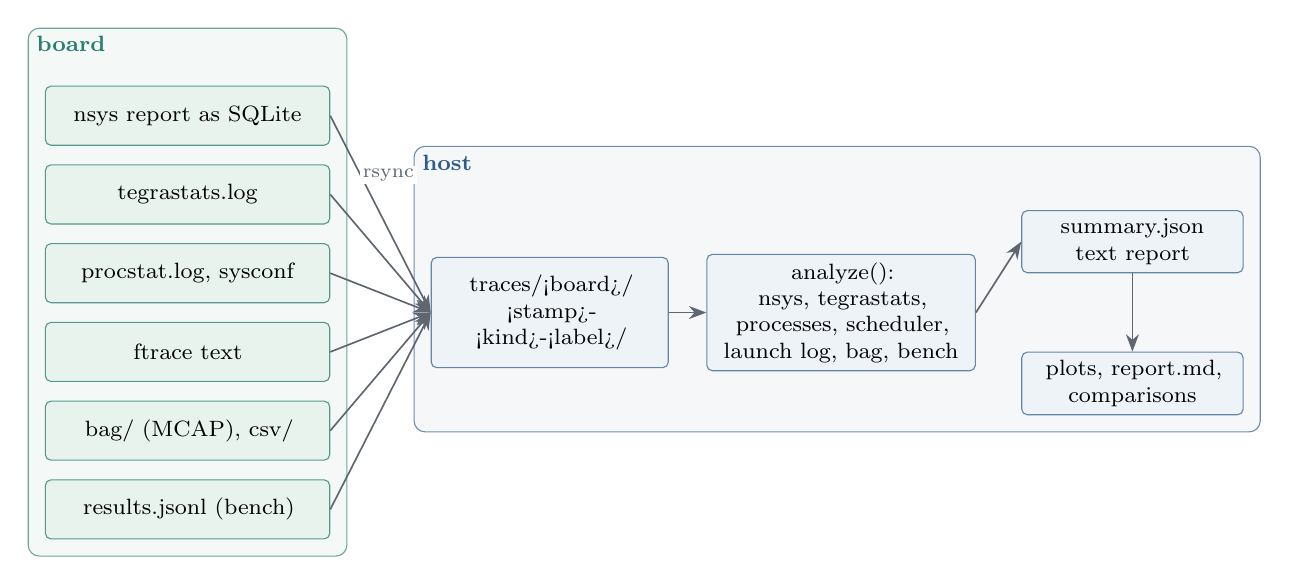
\begin{tikzpicture}[x=1cm,y=1cm]
  \foreach \y/\n/\t in {2.5/a/{\code{nsys} report as SQLite}, 1.5/b/\code{tegrastats.log}, 0.5/c/{\code{procstat.log}, \code{sysconf}},
                        -0.5/d/{ftrace text}, -1.5/e/{\code{bag/} (MCAP), \code{csv/}}, -2.5/f/{\code{results.jsonl} (bench)}}{
    \node[boardbox=34mm] (\n) at (0,\y) {\t};
  }
  \node[hostbox=28mm, minimum height=14mm] (g) at (4.6,0) {\code{traces/<board>/}\\\code{<stamp>-<kind>-<label>/}};
  \node[hostbox=32mm, minimum height=14mm] (h) at (8.3,0) {\code{analyze()}:\\nsys, tegrastats, processes, scheduler, launch log, bag, bench};
  \node[hostbox=26mm] (i) at (12.0,0.9) {\code{summary.json}\\text report};
  \node[hostbox=26mm] (k) at (12.0,-0.9) {plots, \code{report.md},\\comparisons};
  \foreach \n in {a,b,c,d,e,f} \draw[arr] (\n.east) -- (g.west);
  \node[lbl] at (2.55,1.75) {rsync};
  \draw[arr] (g) -- (h);
  \draw[arr] (h.east) -- (i.west);
  \draw[arr] (i) -- (k);
  \begin{scope}[on background layer]
    \node[group=jxbteal, fit={(a)(f)(0,3.4)}] (B) {};
    \node[group=jxbblue, fit={(g)(h)(i)(k)(8.3,1.9)}] (H) {};
  \end{scope}
  \node[glabel=jxbteal] at (B.north west) {board};
  \node[glabel=jxbblue] at (H.north west) {host};
\end{tikzpicture}
\caption{From raw recordings to reports.}\label{fig:tracepipe}
\end{figure}

\paragraph{Measurement lock.} On a shared board, a measurement must not include another user's load (\finding{53}).
Every recording command is wrapped in an advisory lock (\cref{lst:lock}). \code{flock -o} closes the lock's file
descriptor before running the command, so children that outlive it cannot hold the lock; \code{-E 75} gives a distinct
exit code on time-out. Any other tool can take part with \code{flock ~/jxb/.measure.lock <command>}; the
hardware-in-the-loop session that shares the Nano does so.

\begin{lstlisting}[language=Python, caption={The measurement lock (\codeb{locked()} in \codeb{jxb_trace.py}).}, label={lst:lock}]
held = f"echo {q(note)} > {q(lock)}.info; {command}; rc=$?; rm -f {q(lock)}.info; exit $rc"
return (f"flock -n {q(lock)} true 2>/dev/null || echo \"[jxb] {board.name} is busy with another measurement "
        f"($(cat {q(lock)}.info 2>/dev/null || echo 'holder unknown')); waiting up to {timeout} s\"; "
        f"exec flock -o -w {timeout} -E 75 {q(lock)} bash -c {q(held)}")
\end{lstlisting}

\subsection{Nsight Systems}
\code{jxb trace nsys BOARD -- CMD} runs \code{nsys profile --trace cuda,nvtx,osrt,cublas,cudnn} with process-tree CPU
sampling and context-switch tracing~\cite{nsys}, which works without root on a stock board
(\code{perf_event_paranoid=2}; system-wide sampling does not, \finding{45}). \code{--kill 2} ends the profiled process
with SIGINT, so ROS nodes shut down cleanly. The report is exported to SQLite on the board
(\code{nsys export --type sqlite}), and \code{nsys_summary} evaluates it with SQL over the CUPTI tables, for example:
\begin{lstlisting}[language=SQL]
SELECT s.value, count(*), sum(k.end - k.start), max(k.end - k.start)
FROM CUPTI_ACTIVITY_KIND_KERNEL k JOIN StringIds s ON s.id = k.shortName
GROUP BY k.shortName ORDER BY 3 DESC
\end{lstlisting}
The sum of kernel durations overstates the GPU utilization when kernels of several streams overlap. The \textbf{GPU busy
time} is therefore the measure of the union of the kernel intervals (\cref{fig:union}):
\begin{equation}
  B = \Bigl\lvert \bigcup_i\, [s_i, e_i) \Bigr\rvert , \qquad u_{\mathrm{GPU}} = \frac{B}{t_1 - t_0},
\end{equation}
computed in one pass over the intervals sorted by start time: an interval that starts after the current merged
interval ends closes it, otherwise it extends it. $[t_0, t_1]$ is the span covered by kernels, CUDA API calls, OS
runtime calls and NVTX ranges. The summary further contains memory copies by direction, CUDA API calls, NVTX ranges,
OS runtime calls and the hottest leaf functions of the CPU samples. Sections whose tables differ between nsys versions
fail individually and are listed in \code{errors}, while the other sections remain.

\begin{figure}[H]
\centering
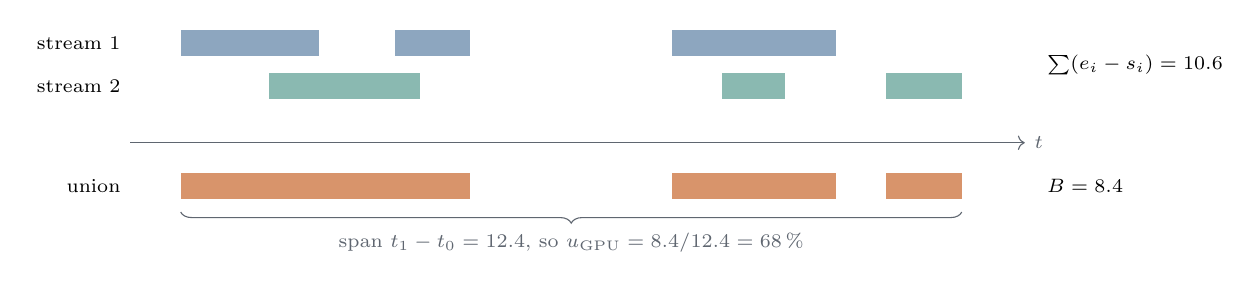
\begin{tikzpicture}[x=0.8cm,y=0.55cm]
  \draw[->, jxbgray] (0,0) -- (14.2,0) node[right, font=\scriptsize]{$t$};
  \node[font=\scriptsize, anchor=east] at (0,2.3) {stream 1};
  \node[font=\scriptsize, anchor=east] at (0,1.3) {stream 2};
  \node[font=\scriptsize, anchor=east] at (0,-1.0) {union};
  \foreach \a/\b in {0.8/3.0, 4.2/5.4, 8.6/11.2}{\fill[jxbblue!55] (\a,2.0) rectangle (\b,2.6);}
  \foreach \a/\b in {2.2/4.6, 9.4/10.4, 12.0/13.2}{\fill[jxbteal!55] (\a,1.0) rectangle (\b,1.6);}
  \foreach \a/\b in {0.8/5.4, 8.6/11.2, 12.0/13.2}{\fill[jxborange!70] (\a,-1.3) rectangle (\b,-0.7);}
  \draw[jxbgray, decorate, decoration={brace, mirror, amplitude=4pt}] (0.8,-1.6) -- (13.2,-1.6)
     node[midway, below=4pt, font=\scriptsize]{span $t_1 - t_0 = 12.4$, so $u_{\mathrm{GPU}} = 8.4/12.4 = 68\,\%$};
  \node[font=\scriptsize, align=left, anchor=west] at (14.4,1.8) {$\sum (e_i - s_i) = 10.6$};
  \node[font=\scriptsize, align=left, anchor=west] at (14.4,-1.0) {$B = 8.4$};
\end{tikzpicture}
\caption{GPU busy time as the measure of the union of kernel intervals; the plain sum counts overlaps twice.}\label{fig:union}
\end{figure}

\subsection{tegrastats}
\code{tegrastats} is JetPack's telemetry tool and needs no root. A line such as the following (abridged, from the stack
recording in \cref{sec:stack}; note the board's clock at 1970)
\begin{lstlisting}
01-15-1970 00:39:37 RAM 1168/7486MB (lfb 17x4MB) CPU [40%@1344,2%@1344,38%@1344,20%@1344,0%@1344,1%@1344]
GR3D_FREQ 0% cpu@49C/49C ... gpu@48.187C/48.25C tj@49C/49C ... VDD_IN 5811mW/5816mW/5821mW VDD_CPU_GPU_CV 1669mW/...
\end{lstlisting}
is parsed by regular expressions into a flat record (memory, swap, load and frequency per core, GPU load and
frequency, memory-controller load, temperature per zone, power per rail), written as CSV and summarized as mean,
minimum and maximum per metric. With the sampling interval $\Delta t$ and the input power samples $P_k$ of rail
\code{VDD_IN}, the energy of a recording is
\begin{equation}
  E = \sum_k P_k\, \Delta t .
\end{equation}
$\Delta t$ is not the nominal \code{--interval}: on the Nano, tegrastats samples every 507.3\,ms for
\code{--interval 500}, 1.5\,\% long (\finding{82}). Its lines carry the board's clock to the second. From 30\,s of
recording on, a least-squares fit of those timestamps over the sample index estimates $\Delta t$ to better than
0.5\,\% (0.1\,\% over 25 minutes), and the fitted value (\code{interval_real_ms}) is used for the time axis and the
energy. Shorter recordings keep the nominal interval, because the fit's error would be as large as the effect.

tegrastats runs on the board host, also in container mode, without inherited standard streams
(\code{< /dev/null > /dev/null 2>&1}), so a leftover can never hold the SSH channel open, and it is stopped by an exit
trap (\finding{62}).

\subsection{Per-process monitoring}
\code{jxb launch --monitor} samples every process of the board once per second (\cref{lst:procmon}). Each \code{T} line
starts a sample; the \code{/proc/<pid>/stat} lines give the parent PID, the user and system CPU ticks
(\code{utime + stime}), the start time and the resident set size. Attribution is by \textbf{ancestry}: \code{R} is the
PID of the session's shell and \code{C} the PID of the init process of its runtime container, and a process belongs to
the session if one of its ancestors is such a root. This is robust against processes of other users that start during
the recording (\finding{53}).

\begin{lstlisting}[language=bash, caption={The per-process sampler (\codeb{PROCMON}).}, label={lst:procmon}]
echo "R $$"; while :; do echo "T $(cut -d" " -f1 /proc/uptime)"
  if [ -n "$JXB_CN" ] && [ -z "$JXB_CP" ]; then
    JXB_CP=$(docker inspect -f "{{.State.Pid}}" "$JXB_CN" 2>/dev/null | grep -v "^0$") && echo "C $JXB_CP"; fi
  cat /proc/[0-9]*/stat 2>/dev/null; sleep 1; done
\end{lstlisting}

For a process with tick counts $k_1, k_2$ at the sample times $t_1, t_2$ and the tick rate $h$ (\code{CLK_TCK}), the
load and the share of a recording of length $T$ are
\begin{equation}
  \mathrm{cpu}(t_2) = 100\,\frac{k_2 - k_1}{h\,(t_2 - t_1)}\ \%, \qquad
  \mathrm{share} = 100\,\frac{k_{\mathrm{last}} - k_{\mathrm{first}}}{h\,T}\ \%,
\end{equation}
where 100\,\% is one core. The share divides by the whole recording, so short-lived processes do not inflate the total,
whereas the mean divides by the process's lifetime. The sampler's own cost is reported separately
(\code{monitor_cpu_pct}, about 1.1\,\% of one core).

\subsection{Kernel tracing}
\code{jxb trace kernel} uses plain ftrace via tracefs~\cite{ftrace}, which every stock kernel provides. The board helper
\code{jxb-ftrace.sh} saves the tracing state (\code{tracing_on}, buffer size, tracer, enabled events,
\code{record-tgid}), enables the requested event groups (scheduler, IRQ, power, system calls, work queues), records or
streams, and \textbf{restores the previous state on every exit}, since the board is shared. Root is required (tracefs is
\code{drwx------}): by default \code{sudo} asks the user for the password in the terminal (\jxb{} never handles
passwords); alternatives are a privileged container (\code{--root docker}) or none.

\code{SchedStats} turns the ftrace text into scheduler statistics in one pass: run time per task (time between being
switched in and out on a CPU), busy time per CPU, context switches and preemptions (\code{prev_state=R}), IRQ and
softirq handler times, and the \textbf{wakeup latency} of every task,
\begin{equation}
  L = t_{\text{switch-in}} - t_{\text{wakeup}},
\end{equation}
reported as p50, p99 and maximum per task. On the board's PREEMPT\_RT kernel this is the quantity that determines the
reaction time of control nodes. The same class drives a live view with per-second statistics.

ftrace keeps a fixed ring buffer per CPU and overwrites the oldest events when it is full. The full SAM stack writes
about 300\,000 events/s with the default presets, so a buffer of 8\,MB per CPU kept only the last 5.9\,s of a 30\,s
recording (\finding{80}). After an overflow, each CPU's data starts at a different time; a wakeup recorded on one CPU
then had its switch-in on another CPU's lost data, which produced spurious delays of 0.1--0.4\,s. \jxb{} therefore
reads the trace header (\code{entries-in-buffer/entries-written}), computes the statistics only over the window that
every CPU covers (from the last \code{CPU N buffer started} marker; \code{SchedStats.reset()} carries the running tasks
over), and reports the share of events it kept together with the buffer that would keep all of them,
$\lceil 1.1\, b\, w / k \rceil$\,MB per CPU for buffer $b$, $w$ events written and $k$ kept. \code{--buffer-mb} sets the
buffer; by default it grows with \code{--duration} from 8 to 32\,MB per CPU. It stays bounded because the board is
shared and its kernel has a bug in memory-cgroup accounting (\finding{79}, \finding{85}).

\subsection{Inference benchmarks}
\code{jxb trace bench BOARD --models M.onnx ...} runs a matrix of backends on the board: ONNX Runtime with the CPU,
CUDA and TensorRT EPs (fp32, fp16 and, for models with Q/DQ nodes, INT8) through \jxb's \code{ort_bench}, and native
TensorRT engines through \code{trtexec} (fp32, fp16, INT8). Each run yields the p50, p90 and p99 latency, the GPU
compute time (trtexec) and the throughput as one JSON line. The summary sorts the backends by p50 and reports the
speed-up against ONNX Runtime's CUDA EP, the \enquote{no TensorRT} baseline,
\begin{equation}
  S = \tilde t_{\text{ort-cuda}} \,/\, \tilde t_{\text{backend}},
\end{equation}
where $\tilde t$ is the median latency. Engines are built on the board, because they are specific to the GPU and the
TensorRT version, and kept for reuse, for example as the SAM node's \code{model:=<...>.engine}.

\subsection{Reports, plots and comparisons}
\code{jxb trace report} prints the summary of a recording, \code{jxb trace plot} renders plots and a Markdown report
with matplotlib in the dev container, and \code{jxb trace compare A B ... --name N} puts several recordings side by
side in \code{traces/compare/N/}; the comparison also lists the board settings that differ between the recordings
(\cref{sec:boardstate}). The figures of \cref{sec:stack} were produced this way.

\subsection{Board state and a common time axis}\label{sec:boardstate}
Each recording captures the board's state at its start and at its end: one shell pipeline of \code{grep -H} over
sysfs, without root, in about 25\,ms. It runs \emph{inside} the measurement lock, so another user's
\code{jetson_clocks} shows. It records the power mode; the CPU policies' governors and limits; every devfreq device
(the GPU, EMC as \code{bwmgr}, the video and vision engines); the CPU idle states and GPU rail gating; fan control and
the thermal zones; and the board's wall clock and uptime. The report flags clocks held at one frequency
(minimum = maximum, the signature of \code{jetson_clocks}) and every setting that differs between start and end;
\code{compare} lists settings that differ between recordings (\finding{73}).

Boards often run without NTP (the Nano's clock is at 1970), so a common time axis needs each board's offset
$\theta = t_{\text{board}} - t_{\text{host}}$. \jxb{} estimates it after each recording over one SSH connection, the
way NTP does: the host sends a line at $t_0$, the board answers with its clock $t_b$, and the answer arrives at
$t_1$. Then
\begin{equation}
  \hat\theta = t_b - \frac{t_0 + t_1}{2}, \qquad |\hat\theta - \theta| \le \frac{t_1 - t_0}{2}.
\end{equation}
The first exchange, which includes the connection setup, is discarded; of eight more, the one with the shortest
round trip is kept. On the lab network the round trip is about 3\,ms, so the error bound is about 1.5\,ms; five
estimates agreed within 0.39\,ms (\finding{77}). With $\hat\theta$, and with the board's wall clock $w_0$ and uptime
$u_0$ at the start, board times (nsys, bag stamps, rate probes) map to host time as
$t_{\text{host}} = t_{\text{board}} - \hat\theta$, and uptimes (per-process samples) as
$t_{\text{host}} = (w_0 - \hat\theta) + (u - u_0)$.

\subsection{Timelines}\label{sec:timeline}
\code{jxb trace perfetto} writes recordings as one timeline in the Chrome JSON trace event format, which the Perfetto
UI opens. Each recording becomes one process, a group of tracks: its board state as an instant event; counter tracks
for tegrastats (CPU, GPU, RAM, board power, junction temperature), each session process's CPU and RSS, the memory
counters, topic rates and numeric bag topics; and slices for nsys's GPU kernels (one track per CUDA stream) and NVTX
ranges, and ROS~2 callbacks (\code{--ros-trace}) per thread (\cref{sec:rostrace}). Times are the host's (\cref{sec:boardstate}), so recordings of several boards made at once line up, and a
fan-out recording writes the merged timeline by itself. Two independent sources agree in a recorded launch: the
first inference (bag, board clock) is at $+5.09$\,s, the rise of GPU load (tegrastats, start plus sampling interval)
at $+5.00$\,s; nsys kernels fall inside their NVTX ranges (\finding{77}). Perfetto's UI loads \code{?url=} traces only
from \code{127.0.0.1:9001} (its content security policy), so files are opened with ``Open trace file''.

\subsection{ROS 2 tracing}\label{sec:rostrace}
\code{jxb launch --ros-trace} and \code{jxb trace ros} record ROS~2's own tracepoints, which the \code{tracetools}
package compiles into rcl and rclcpp; the libraries link against LTTng's userspace tracer. The Nano ships lttng-tools
2.13, and \code{lttng create} as an ordinary user starts a session daemon for that user, so this needs neither root nor
packages (\finding{83}). The wrapper creates a session with one userspace channel (8 $\times$ 1\,MB sub-buffers per
CPU), enables \code{ros2:*} with the context \code{vpid}, \code{vtid} and \code{procname}, runs the launch, stops and
destroys the session and converts the trace with \code{babeltrace --clock-seconds}. \code{RosTrace} resolves what every
callback serves from the setup events: nodes, subscriptions (\code{rcl_subscription_init} $\to$
\code{rclcpp_subscription_init} $\to$ \code{rclcpp_subscription_callback_added}), timers with period and node,
services, publishers and the C++ symbol (\code{rclcpp_callback_register}). The session therefore has to start before
the nodes do, which \code{--ros-trace} ensures. From the run events it computes each callback's execution intervals per
thread, publish counts per topic and, for each taken message, its age (\code{rmw_take}: take time minus the DDS source
timestamp, i.e.\ transport plus queueing), all on the board's clock, which the timeline maps to the host's
(\cref{sec:boardstate}). In SAM's detector this showed images taken 0.32\,s after they were published: a keep-last-10
queue drained by \code{spin_some()} at 5\,Hz (\finding{83}). Container mode is not supported yet; the runtime container
would need the user's LTTng socket directory and the session daemon's shared memory.

% ======================================================================================================== 8
\section{VS Code integration}\label{sec:vscode}
Like the Renesas RDK~\cite{renesas-vscode}, \jxb{} integrates with VS Code through tasks and debug configurations, but
every task only calls \jxb, so the terminal and the editor run the same code (R6). \code{jxb vscode init -w WS} writes a
multi-root workspace file \code{vscode/<ws>.code-workspace} (the ROS workspace plus the \jxb{} repository); the
workspace's own \code{.vscode/} stays untouched. What the tasks act on is set in the workspace settings, which take the
role of the RDK's \code{settings.json} variables: \code{jxb.profile}, \code{jxb.mode}, \code{jxb.board},
\code{jxb.package}, \code{jxb.executable}, \code{jxb.launchPackage}, \code{jxb.launchFile}, \code{jxb.launchArgs},
\code{jxb.launchWith}, \code{jxb.bagTopics}, \code{jxb.benchModels}, \code{jxb.gdbPort} and \code{jxb.traceSeconds}.
Tasks reference them as \codeb{${config:jxb.board}}; running \code{init} again regenerates tasks and configurations and
keeps the settings (\cref{tab:tasks}).

\begin{table}[H]
\centering\small
\caption{Generated VS Code tasks.}\label{tab:tasks}
\begin{tabularx}{\textwidth}{@{}lX@{}}
\toprule
Group & Tasks (all prefixed \enquote{jxb:}) \\
\midrule
build & build (default build task, \code{$gcc} problem matcher), build package (debug info), \dots{} + deploy \\
run & deploy, run node on board, launch on board, launch + monitor (recorded), launch + monitor + bag (recorded), ssh to board \\
debug & gdbserver node, cuda-gdbserver node, gdbserver node in launch, stop gdbserver launch, and per further board gdbserver node (\code{<board>}) \\
trace & trace nsys node, trace nsys launch, tegrastats live, kernel trace, kernel trace live (top), trace report, trace plot, benchmark models \\
checks & board check, test suite on board, container shell \\
\bottomrule
\end{tabularx}
\end{table}

The debug configurations (a node, a node in a launch file, a node with CUDA code) use \code{cppdbg} with
\code{miDebuggerPath} set to \code{toolchain/bin/jxb-gdb} (which
runs \code{jxb gdb} with the profile's sysroot) and \code{miDebuggerServerAddress} \codeb{127.0.0.1:${config:jxb.gdbPort}}.
Their \code{preLaunchTask} starts \code{jxb debug --server-only} as a \textbf{background task}. VS Code must know when
the server is ready; a problem matcher with a never-matching pattern whose \code{beginsPattern} and \code{endsPattern}
are \code{Listening on port} signals exactly that. For a node in a launch file, a \code{postDebugTask} terminates the
launch task through an input of type \code{command} (\code{workbench.action.tasks.terminate}). The flow was verified by
replaying the generated configuration over gdb's machine interface the way \code{cppdbg} drives it (\finding{47}).

The CUDA configuration passes \code{--jxb-cuda}, so the wrapper runs \code{cuda-gdb} (\cref{sec:debug}). With several
\code{--board} options, \code{init} adds a gdbserver task and a debug configuration per further board, each on its
board's \code{gdb_port}, and a compound ``jxb: debug node on all boards'' that starts them together. Every session
forwards its board's gdbserver to \code{127.0.0.1:<port>} on the host, so \code{init} refuses boards that share a port.

% ======================================================================================================== 9
\section{Evaluation}\label{sec:eval}

\subsection{Setup}
\begin{table}[H]
\centering\small
\caption{Experimental setup.}\label{tab:setup}
\begin{tabularx}{\textwidth}{@{}lX@{}}
\toprule
Host & x86\_64, 20 cores, 15\,GB RAM, Docker, Arch-based Linux \\
Board & Jetson Orin Nano 8\,GB, JetPack 7.2.1 (L4T 39.2.1), 25\,W mode, GPU at 918\,MHz, PREEMPT\_RT kernel, NVMe \\
Workload & SAM ROS~2 workspace (snapshot 7552ca7f); detector models S0 (YOLO, fp32, $1\times3\times608\times960$) and quantized variants \\
Input & synthetic camera \code{jxb_image_pub.py}, 30\,fps, $1280\times800$ for the stack \\
\bottomrule
\end{tabularx}
\end{table}
The board is shared with other users; all measurements ran under the measurement lock. Each configuration was recorded
once for 40--120\,s unless stated otherwise, so the numbers are indicative baselines rather than statistically
established results (\cref{sec:threats}).

\subsection{Build side}
\begin{table}[H]
\centering\small
\caption{Sysroots, test results and SAM workspace per profile.}\label{tab:build}
\begin{tabularx}{\textwidth}{@{}lrrl>{\raggedright\arraybackslash}X@{}}
\toprule
Profile & Packages & Size & Tests (host / board) & SAM workspace \\
\midrule
\code{jp721-jazzy} & 944 & 16\,GB & 12 / 8 & all but 2 packages, which need Kilted APIs (\finding{15}) \\
\code{jp721-kilted} & 995 & 16\,GB & 14 / 9 & all but \code{pylon_camera_package} (Basler SDK) and the vendored \code{micro_ros_agent} (\finding{54}) \\
\code{jp721-lyrical-isaac} & 1068 & 19\,GB & 15 / 10 & all but \code{localization_package} (Lyrical tf2, \finding{28}) and Pylon; \code{oak_camera_package} with \jxb's depthai \\
\code{jp721-lyrical} & 1100 & 17\,GB & 12 / container & all but \code{localization_package} and Pylon (\finding{28}) \\
\bottomrule
\end{tabularx}
\end{table}
The SAM workspace cross-builds with Kilted in 2:18\,min cold and 1:14\,min with a warm ccache (\finding{19}), and
\code{jxb-elfcheck} reports no linkage problem. A sysroot rebuild from the cache takes about one minute. A fully
parallel build initially ran out of memory on the 15\,GB host: colcon runs \code{make -j<cores>} per package, so six
parallel packages meant up to 120 compiler processes (\finding{54}); \code{MAKEFLAGS=-j4} with three parallel packages
builds all 26 packages in 3.5\,min.

\subsection{Inference baselines}
\Cref{tab:bench,fig:bench} give the latency of the SAM detector models per backend.

\begin{table}[H]
\centering\small
\caption{Inference benchmark on the Orin Nano ($1\times3\times608\times960$ input). Speed-up relative to ONNX Runtime's
CUDA EP.}\label{tab:bench}
\setlength{\tabcolsep}{4.5pt}
\begin{tabular}{@{}llrrrr@{}}
\toprule
Model & Backend & p50 [ms] & p99 [ms] & Rate [1/s] & Speed-up \\
\midrule
S0 fp32 & ONNX Runtime CPU & 355.0 & 515.1 & 2.5 & 0.10 \\
 & ONNX Runtime CUDA EP & 35.1 & 36.1 & 28.5 & 1.00 \\
 & ONNX Runtime TensorRT EP fp32 & 22.6 & 27.3 & 43.8 & 1.56 \\
 & \code{trtexec} fp32 & 21.9 & 25.5 & 45.2 & 1.60 \\
 & ONNX Runtime TensorRT EP fp16 & 11.9 & 14.1 & 82.1 & 2.95 \\
 & \code{trtexec} fp16 & \textbf{10.8} & 12.0 & 90.9 & 3.24 \\
\midrule
P1 PTQ INT8 & \code{trtexec} INT8 & 9.10 & 9.49 & 109.1 & 5.20 \\
S2 QAT INT8 & \code{trtexec} INT8 & 9.02 & 9.78 & 110.2 & 5.25 \\
Q4 full INT8 & \code{trtexec} INT8 & 8.92 & 9.19 & 111.4 & 5.36 \\
S3 QAT INT8 (n-model) & \code{trtexec} INT8 & \textbf{6.75} & 7.18 & 146.6 & 3.98 \\
\bottomrule
\end{tabular}
\end{table}

\begin{figure}[t]
\centering
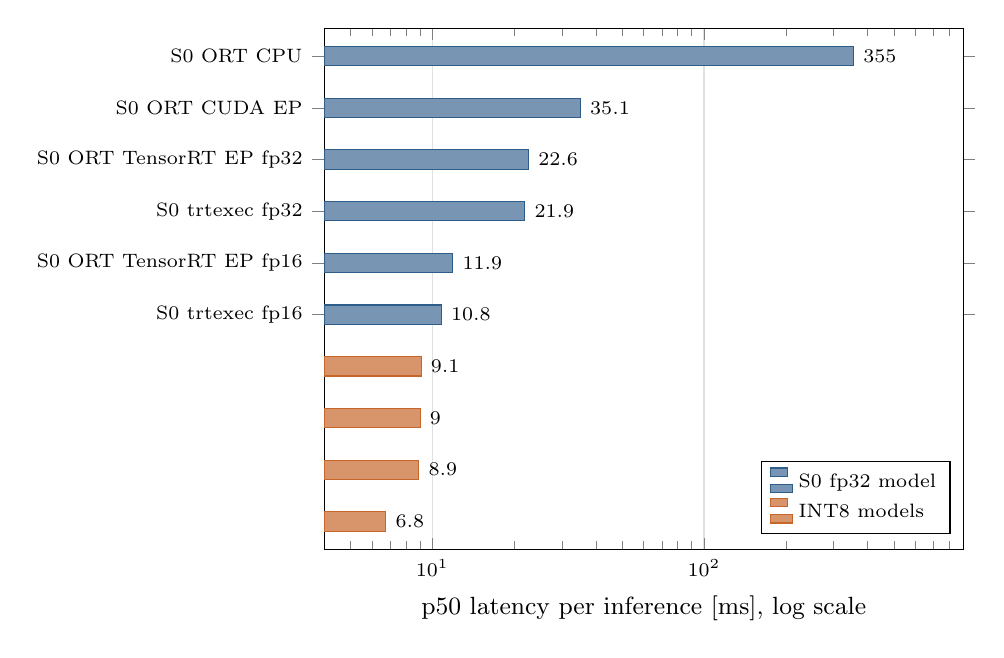
\begin{tikzpicture}
\begin{axis}[
  xbar, xmode=log, log origin=infty, width=0.80\textwidth, height=8.2cm, xmin=4, xmax=900,
  bar width=7pt, y dir=reverse, ytick=data, enlarge y limits=0.06,
  symbolic y coords={S0 ORT CPU,S0 ORT CUDA EP,S0 ORT TensorRT EP fp32,S0 trtexec fp32,S0 ORT TensorRT EP fp16,
    S0 trtexec fp16,P1 PTQ trtexec INT8,S2 QAT trtexec INT8,Q4 full INT8 trtexec,S3 QAT n-model trtexec INT8},
  yticklabel style={font=\scriptsize}, xticklabel style={font=\scriptsize},
  xlabel={p50 latency per inference [ms], log scale}, xlabel style={font=\small},
  point meta=rawx, nodes near coords={\pgfmathprintnumber[fixed,precision=1]{\pgfplotspointmeta}},
  nodes near coords style={font=\scriptsize, anchor=west}, xmajorgrids, grid style={jxbgray!20},
  legend style={font=\scriptsize, at={(0.98,0.03)}, anchor=south east}, legend cell align=left]
\addplot[fill=jxbblue!65, draw=jxbblue, bar shift=0pt] coordinates {
  (355.0,S0 ORT CPU) (35.1,S0 ORT CUDA EP) (22.6,S0 ORT TensorRT EP fp32) (21.9,S0 trtexec fp32)
  (11.9,S0 ORT TensorRT EP fp16) (10.8,S0 trtexec fp16)};
\addplot[fill=jxborange!70, draw=jxborange, bar shift=0pt] coordinates {
  (9.10,P1 PTQ trtexec INT8) (9.02,S2 QAT trtexec INT8) (8.92,Q4 full INT8 trtexec) (6.75,S3 QAT n-model trtexec INT8)};
\legend{S0 fp32 model, INT8 models}
\end{axis}
\end{tikzpicture}
\caption{Median inference latency per backend (log scale).}\label{fig:bench}
\end{figure}

Three observations follow. (1)~TensorRT is the decisive factor: fp16 engines are $3.2\times$ faster than ONNX
Runtime's CUDA EP. (2)~ONNX Runtime's TensorRT EP comes within about 10\,\% of \code{trtexec} (11.9 vs.\ 10.8\,ms), so an
application can keep the ONNX Runtime API and still obtain most of the benefit. (3)~INT8 reduces the latency by only
about 17\,\% relative to fp16 for the s-sized model; the smaller n-model is the larger lever. Without TensorRT, the Q/DQ
models are \emph{slower} than fp32 (CUDA EP 47\,ms vs.\ 35\,ms), because the quantization nodes are executed as fake
quantization. An Nsight Systems trace of the CUDA EP run explains part of its cost: the inputs come from pageable host
memory and are staged synchronously (\code{cudaMemcpyAsync} took 962\,ms of API time for 430\,MB that the GPU copied in
55\,ms), and layout-conversion kernels take 6.4\,\% of the GPU time (\finding{46}).

\subsection{The SAM detector node}
In the ROS node (\cref{fig:detector}), inference takes 46.4\,ms (p50) with ONNX Runtime's CUDA EP, 17.2\,ms with a
TensorRT fp16 engine and 15.1\,ms with an INT8 (QAT) engine. The TensorRT backends also halve the session's memory
(1.79 vs.\ 0.85\,GB) and save about 1\,W (6.9 vs.\ 5.9\,W). The node adds 6--11\,ms around the engine, and it runs a fixed
5\,Hz loop, so the GPU is busy only 4--13\,\% of the time; the detection rate is bounded by that loop, not by the GPU
(\finding{50}). Jazzy and Kilted give the same results within noise; under Lyrical (Isaac Buildfarm, native) memory and
CPU are the same as well (1.83\,GB with ONNX Runtime, 0.89\,GB with TensorRT); its inference times were not recorded in
that campaign, because bag recording failed with the Lyrical runtimes (fixed since, \finding{68}: a later run gives a
median of 17.3\,ms). The runtime container
differs from the first native run by $+0.6$\,ms and $+0.14$\,GB, but a second native run differs from it by as much
($+0.5$\,ms, $+0.14$\,GB): the container's cost is within run-to-run variation (see the measurement report,
\code{measurements.pdf}).

\begin{figure}[t]
\centering
\pgfplotsset{detector/.style={xbar, width=0.40\textwidth, height=5.2cm, bar width=7pt, y dir=reverse, ytick=data,
  enlarge y limits=0.12, xmin=0, symbolic y coords={ORT CUDA EP,TRT fp16,TRT INT8 QAT,TRT fp16 Kilted,TRT fp16 container},
  yticklabel style={font=\scriptsize}, xticklabel style={font=\scriptsize}, xlabel style={font=\scriptsize},
  nodes near coords, nodes near coords style={font=\scriptsize, anchor=west}, xmajorgrids, grid style={jxbgray!20},
  cycle list={{fill=jxbteal!60, draw=jxbteal}}}}
\begin{subfigure}[t]{0.49\textwidth}\centering
\begin{tikzpicture}\begin{axis}[detector, xmax=68, xlabel={inference time, mean [ms]}]
\addplot coordinates {(53.7,ORT CUDA EP) (17.3,TRT fp16) (15.2,TRT INT8 QAT) (17.3,TRT fp16 Kilted) (17.9,TRT fp16 container)};
\end{axis}\end{tikzpicture}
\end{subfigure}\hfill
\begin{subfigure}[t]{0.49\textwidth}\centering
\begin{tikzpicture}\begin{axis}[detector, xmax=2300, xlabel={session RSS [MB]}, ymajorticks=false]
\addplot coordinates {(1791,ORT CUDA EP) (854,TRT fp16) (853,TRT INT8 QAT) (854,TRT fp16 Kilted) (1009,TRT fp16 container)};
\end{axis}\end{tikzpicture}
\end{subfigure}

\vspace{2mm}
\begin{subfigure}[t]{0.49\textwidth}\centering
\begin{tikzpicture}\begin{axis}[detector, xmax=8.8, xlabel={board power, mean [W]}]
\addplot coordinates {(6.88,ORT CUDA EP) (5.89,TRT fp16) (5.74,TRT INT8 QAT) (5.95,TRT fp16 Kilted) (5.99,TRT fp16 container)};
\end{axis}\end{tikzpicture}
\end{subfigure}\hfill
\begin{subfigure}[t]{0.49\textwidth}\centering
\begin{tikzpicture}\begin{axis}[detector, xmax=17.5, xlabel={GPU load, mean [\%]}, ymajorticks=false]
\addplot coordinates {(13.2,ORT CUDA EP) (4.2,TRT fp16) (4.7,TRT INT8 QAT) (6.1,TRT fp16 Kilted) (6.8,TRT fp16 container)};
\end{axis}\end{tikzpicture}
\end{subfigure}
\caption{SAM's \codeb{object_detection} node with the synthetic camera: the first three rows are Jazzy natively, the last
two Kilted natively and in the runtime container (\codeb{jxb trace compare}).}\label{fig:detector}
\end{figure}

\subsection{The full SAM stack}\label{sec:stack}
The complete stack (\code{launch/launch.py module:=parking}: core, object detection, parking and traffic lights; Kilted;
TensorRT fp16 detector) ran for 120\,s with the synthetic camera at 30\,fps, natively and in the runtime container
(\cref{tab:stack}).

\begin{table}[H]
\centering\small
\caption{The SAM stack on the Orin Nano (120\,s each). CPU in cores (1.0 = one core fully used).}\label{tab:stack}
\setlength{\tabcolsep}{3.5pt}
\begin{tabular}{@{}lrrrrrr@{}}
\toprule
Configuration & Proc. & CPU & RSS [GB] & GPU mean/max [\%] & Power [W] & $T_{\max}$ [\si{\celsius}] \\
\midrule
native, TensorRT fp16 & 12 & 2.83 & 2.11 & 12.6 / 84 & 8.36 & 53.0 \\
container, TensorRT fp16 & 12 & 2.75 & 2.07 & 12.5 / 88 & 8.32 & 53.2 \\
native, ONNX Runtime CUDA EP & 12 & 2.93 & 2.92 & 26.8 / 99 & 9.39 & 54.5 \\
native, one process per node & 18 & 2.36 & 1.92 & 13.5 / 88 & 8.11 & 53.6 \\
\bottomrule
\end{tabular}
\end{table}

All processes started and stopped cleanly in every configuration. The composable-node container that hosts the image
pipeline dominates (1.6 cores, 534\,MB, \cref{fig:stackcpu}); the detector takes 0.33 cores and 772\,MB, the synthetic
camera 0.36 cores. Lane points are produced at 23\,Hz and undistorted images at 20--23\,Hz from the 30\,fps input, so the
image pipeline does not keep up with the camera; detections arrive at the node's 5\,Hz. In the loaded system, the
detector's median inference time rises from 17\,ms (alone) to 25\,ms. An Nsight Systems trace of the stack shows the GPU
busy 6.2\,\% of the time, with 2.86\,GB host-to-device and 3.10\,GB device-to-host copies in 46\,s: the pipeline moves
images between CPU and GPU memory in every stage. \Cref{fig:stackteg,fig:stackproc} show the recorded time series.

A kernel trace of the stack (\code{jxb trace kernel}, same setup, \finding{80}) shows where the CPU time outside the nodes
goes. Over the 4.4\,s that every CPU's ring buffer covers there are 75\,600 context switches per second and each CPU is
about 54\,\% busy. Executor and DDS threads wait 3--7\,\si{\micro\second} (p50) and 0.1--1.3\,ms (p99) for a CPU after a wakeup,
with single outliers up to 78\,ms. nvmap's page-zeroing kernel thread \code{nvmap-bz} takes 0.39 cores: the kernel side
of the image pipeline's per-frame device allocations, about 95 \code{cudaMalloc}/\code{cudaFree} pairs per second in
Nsight Systems (\finding{64}). DDS moving the camera images over loopback costs 0.19 cores in \code{NET_RX} softirqs and
0.17--0.20 cores in each receive thread. Reusing GPU buffers would save about half a core.

\begin{figure}[t]
\centering
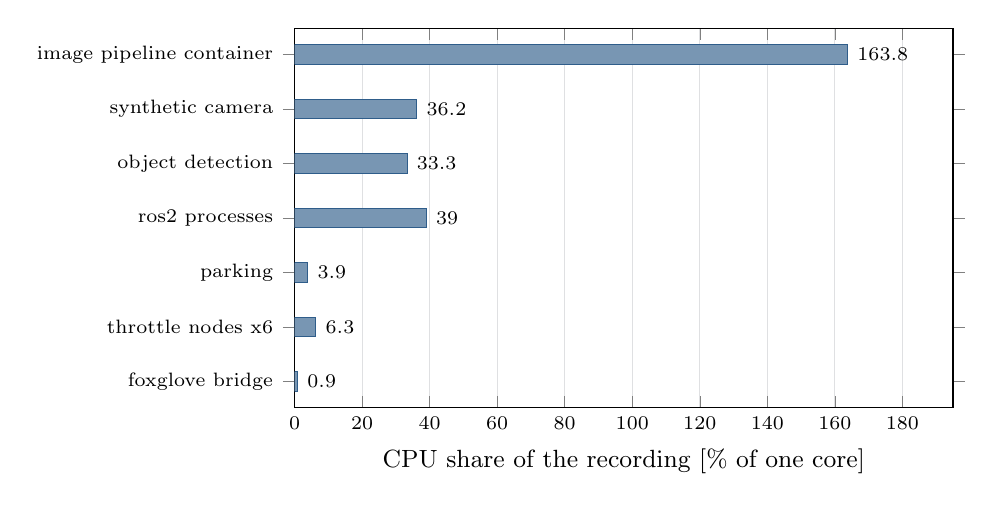
\begin{tikzpicture}
\begin{axis}[
  xbar, width=0.82\textwidth, height=6.4cm, bar width=7pt, y dir=reverse, ytick=data, enlarge y limits=0.08,
  xmin=0, xmax=195, symbolic y coords={image pipeline container,synthetic camera,object detection,ros2 processes,parking,
    throttle nodes x6,foxglove bridge},
  yticklabel style={font=\scriptsize}, xticklabel style={font=\scriptsize},
  xlabel={CPU share of the recording [\% of one core]}, xlabel style={font=\small},
  nodes near coords, nodes near coords style={font=\scriptsize, anchor=west}, xmajorgrids, grid style={jxbgray!20}]
\addplot[fill=jxbblue!65, draw=jxbblue] coordinates {
  (163.8,image pipeline container) (36.2,synthetic camera) (33.3,object detection)
  (39.0,ros2 processes) (3.9,parking) (6.3,throttle nodes x6) (0.9,foxglove bridge)};
\end{axis}
\end{tikzpicture}
\caption{CPU share per process of the SAM stack (native, TensorRT fp16).}\label{fig:stackcpu}
\end{figure}

\begin{figure}[p]
\centering
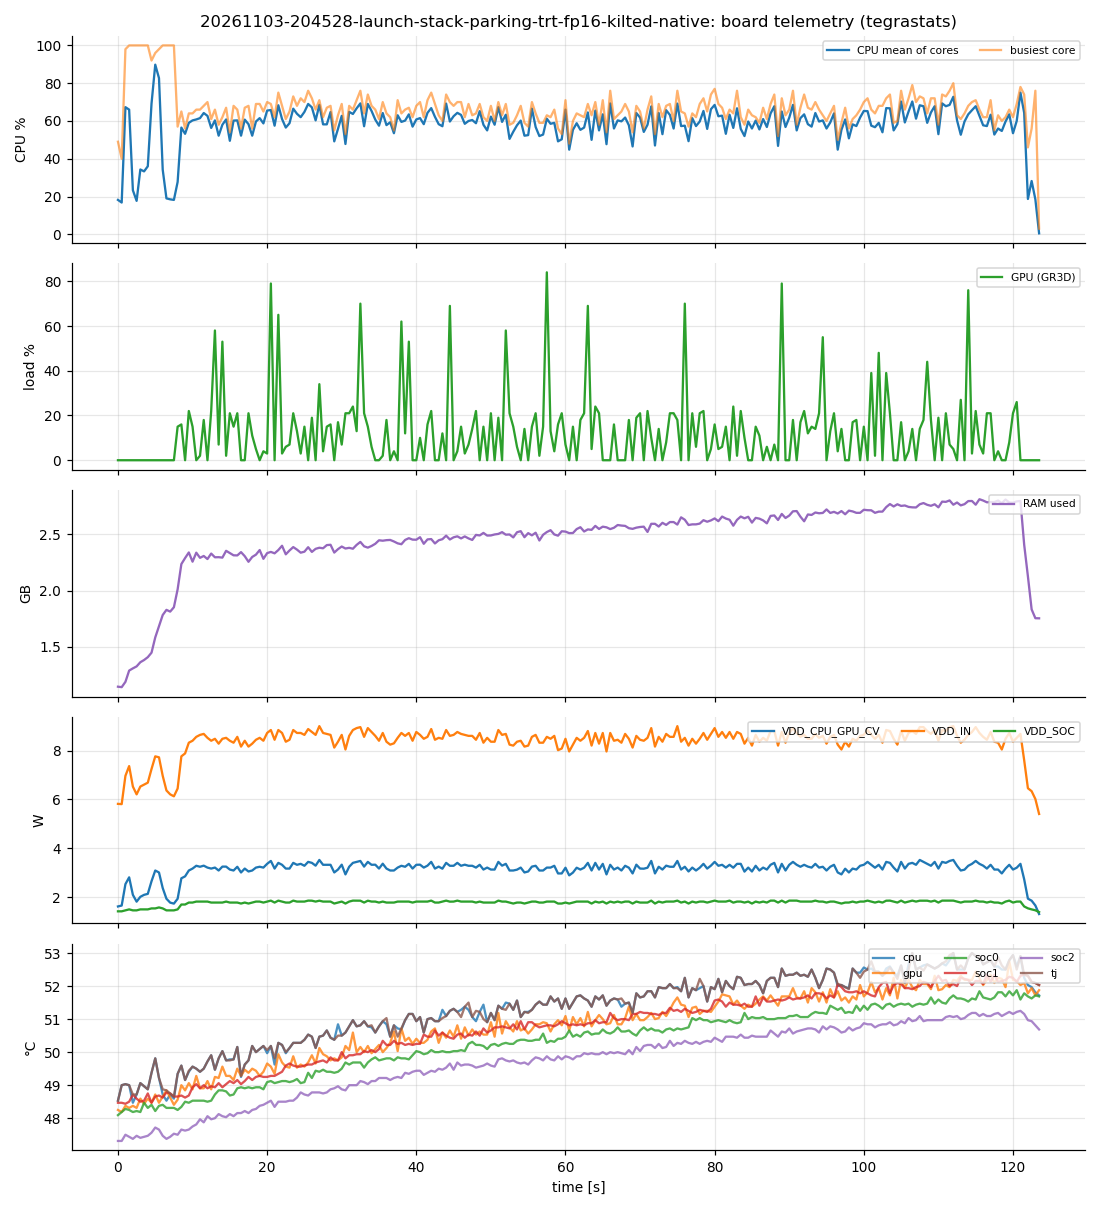
\includegraphics[width=0.80\textwidth]{stack-tegrastats.png}
\caption{tegrastats of the stack run (native, TensorRT fp16): CPU, GPU, memory, power rails and temperatures over
time, as rendered by \codeb{jxb trace plot}.}\label{fig:stackteg}
\end{figure}

\begin{figure}[t]
\centering
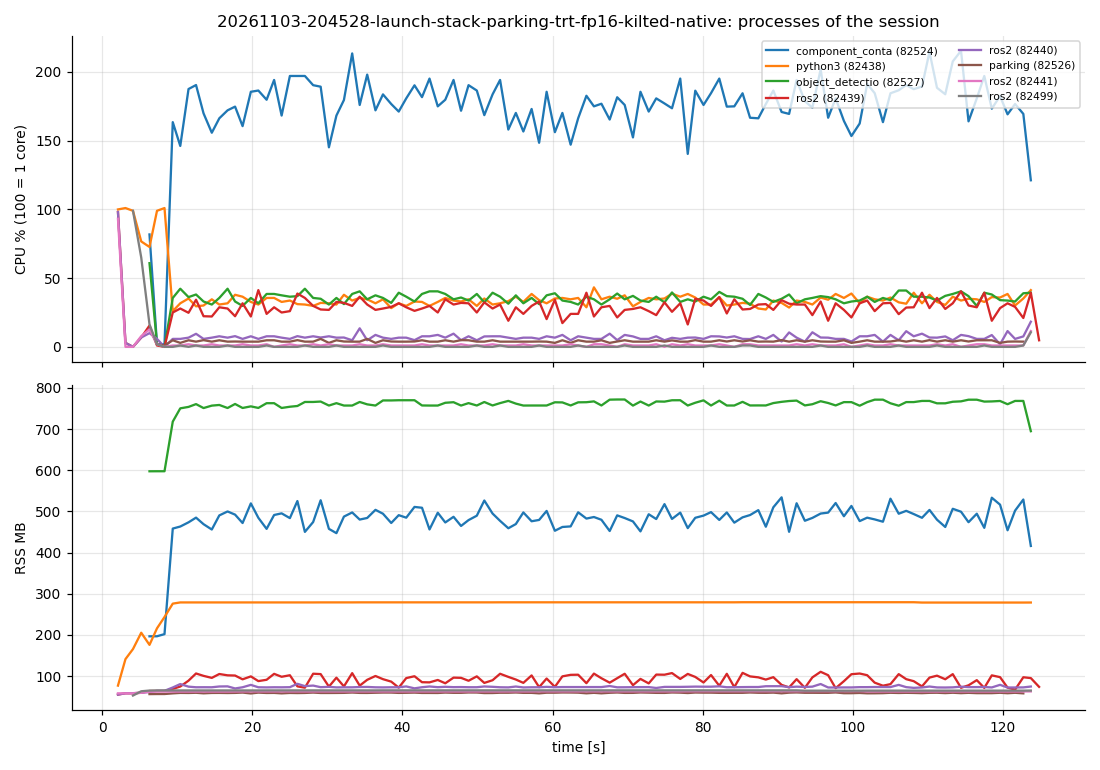
\includegraphics[width=0.86\textwidth]{stack-processes.png}
\caption{CPU (100 = one core) and resident memory of the stack's processes over time.}\label{fig:stackproc}
\end{figure}

\subsection{Discussion and threats to validity}\label{sec:threats}
The results support three conclusions about the system. First, the cross-built binaries behave like native builds:
all tests pass on the board, and the SAM stack runs unchanged under three ROS distributions. Second, container mode is
a viable alternative to native execution: the differences ($+0.6$\,ms inference, $+0.14$\,GB, $\pm3\,\%$ CPU) are
no larger than those between two native runs. Third, the observability pipeline is cheap enough for routine use (about 1\,\% of a
core).

The measurements have limitations. Each configuration was recorded once, on one board, which other users shared; the
lock serializes measurements, but not, for example, the thermal history. The synthetic camera replaces real sensors,
so the planning and control chain stays idle without odometry. Clock and thermal state were recorded but not
controlled. The numbers are baselines for comparisons on this platform, not general performance claims.

% ======================================================================================================== 10
\section{Challenges and lessons learned}\label{sec:challenges}
Of the 62 findings in \code{docs/findings.md}, those that describe problems fall into seven groups. For each group we
state symptoms, root causes and resolutions, and the general lesson.

\subsection{CUDA cross-compilation}
\begin{itemize}
  \item \textbf{Layout change.} CUDA 13 on Orin uses \code{targets/sbsa-linux} (\finding{2}); \jxb{} adds the old name
        as an alias for older CMake versions.
  \item \textbf{Probing.} \code{FindCUDAToolkit} probes \code{nvcc} without flags and picked up x86 include directories
        for C++-only targets (\finding{5}); the image's toolkit was made target-only.
  \item \textbf{Missing sysroot flag.} CMake passes no \code{--sysroot} when the host compiler links CUDA targets
        (\finding{6}).
  \item \textbf{A compiler bug.} CUDA 13.2's CCCL headers declare specializations in a form that GCC 13/14 reject when
        nvcc re-emits them (\finding{22}); the fix suggested upstream is insufficient for \code{.cu} files, a
        namespace-scoped declaration works.
  \item \textbf{Legacy modules.} \code{FindCUDA} takes the target directory only from an environment variable
        (\finding{31}).
\end{itemize}
\begin{lesson}\textbf{Lesson.} Make the defaults of every tool correct for the target instead of relying on flags; check
the target layout of every new JetPack major release.\end{lesson}

\subsection{Sysroot semantics}
\begin{itemize}
  \item Alternatives (\finding{43}), literal \code{ln -s} (\finding{13}) and a boot-time service (\finding{26}) create
        files that builds need.
  \item Key formats (\finding{16}) and pins (\finding{17}) must be reproduced exactly.
  \item Symbolic links must be relative, and CMake must resolve them before computing prefixes (\finding{39}).
  \item Toolchain files are read more than once (\finding{33}): use idempotent \code{list(APPEND)}, never \code{set()}.
\end{itemize}
\begin{lesson}\textbf{Lesson.} Enumerate the side effects of maintainer scripts instead of executing them, and skip what
cannot be determined statically rather than guessing.\end{lesson}

\subsection{Binary portability}
\begin{itemize}
  \item Absolute \code{DT_NEEDED} entries from libraries without \code{SONAME} (\finding{44}) are invisible to a check that
        runs where the path exists.
  \item Build-time paths in generated files: colcon setup scripts and ament's \code{parent_prefix_path} record the sysroot
        path (\finding{37}); they are rewritten after every build.
  \item Python extension suffixes (\finding{12}) and CPU models for emulated tests (\finding{25}).
\end{itemize}
\begin{lesson}\textbf{Lesson.} Verify binaries under the target's view of the file system, not the host's.\end{lesson}

\subsection{Board runtime}
\begin{itemize}
  \item Essential packages are never dependencies, so a sysroot has no shell until they are requested (\finding{48}).
  \item Group names versus numbers in containers whose image is a sysroot (\finding{48}).
  \item Undeclared run-time dependencies in launch files (\finding{52}, \finding{60}) and system Python modules of another
        distribution (\finding{61}).
  \item Incomplete packages break sourcing a whole workspace (\finding{57}); Git LFS pointers silently replace data
        (\finding{51}).
\end{itemize}
\begin{lesson}\textbf{Lesson.} A runtime assembled from declared dependencies is a strict test of those declarations;
treat its failures as bugs of the workspace, not of the runtime.\end{lesson}

\subsection{Process lifecycle on remote boards}
Remote processes outlive their controllers in many ways: an early-dying launch leaves its nodes behind, \code{pkill -f}
hits the wrong processes, and background tools inherit SSH file descriptors (\finding{58}, \finding{62}).
\begin{lesson}\textbf{Lesson.} Manage process groups, not processes; never match command lines; give background tools no
inherited standard streams; and make cleanup part of every exit path (traps).\end{lesson}

\subsection{Shared hardware}
Overlapping measurements (\finding{53}) led to the measurement lock and ancestry-based attribution. More seriously, the
Nano reset about 3\,s into the first run of ONNX Runtime's CUDA EP inside the runtime container, while the EP was
initializing (\finding{56}). Nothing unusual preceded it (1.5\,GB memory used, 49\,\si{\celsius}, 6.7\,W), and the
combination stayed excluded from container runs until root was available. pstore then showed a kernel panic in
\code{kswapd0} (\finding{79}): page reclaim freed buffer heads whose memory-cgroup accounting pointed to an invalid
address (\code{obj_cgroup_uncharge} $\to$ \code{refill_obj_stock}) on the PREEMPT\_RT kernel. It was a kernel bug; the
container's library loading only supplied the memory pressure.
\begin{lesson}\textbf{Lesson.} On shared hardware, an unexplained fault is a policy decision as much as a bug: exclude the
configuration, document it, and keep the evidence. pstore keeps it across the reboot.\end{lesson}
Two more resets followed; the third showed the same fault, reached from an RCU callback instead of reclaim
(\finding{85}): the per-CPU cgroup object stock holds a corrupted pointer, and any accounted free can hit it.
Consequences for \jxb{}: SSH keepalives, a clear message when a board resets during a command, and crash
detection in \code{jxb board check}.
Two more consequences of sharing: another session may run \code{jetson_clocks}, so recordings note the board's state and
flag fixed or changed clocks (\finding{73}); and GPU debugging (group \code{debug}, \finding{75}, \finding{81}) and kernel
tracing (root) are one-time decisions of the board's owners, which \jxb{} names instead of working around.

\subsection{Upstream issues found}
\begin{table}[H]
\centering\small
\caption{Issues in upstream components found during the work.}\label{tab:upstream}
\begin{tabularx}{\textwidth}{@{}lXl@{}}
\toprule
Component & Issue & Finding \\
\midrule
ROS~2 rosidl & \code{file(STRINGS)} without \code{ENCODING UTF-8} breaks non-ASCII workspace paths & \finding{11} \\
CUDA 13.2 CCCL & specialization outside its namespace, rejected by GCC 13/14 & \finding{22} \\
ONNX Runtime & released aarch64 CUDA EP has no \code{sm_87} code; release CMake configuration paths & \finding{8}, \finding{9} \\
SAM & \code{CMAKE_CUDA_ARCHITECTURES} set unconditionally without 87; \code{ekf_core} not installed under Lyrical; hard-coded plugin path & \finding{18}, \finding{55} \\
Lyrical tf2 & \code{tf2/LinearMath/Quaternion.h} removed (only \code{.hpp}) & \finding{28} \\
ONNX Runtime C++ API & \code{GetInputTypeInfo(i).GetTensorTypeAndShapeInfo()} is a view into a temporary & \finding{41} \\
\bottomrule
\end{tabularx}
\end{table}

% ======================================================================================================== 11
\section{Implementation process}\label{sec:process}

\subsection{Timeline}
\Cref{fig:timeline} shows the phases. \textbf{Phase~0} (decisions): a first scaffold from 2026-10-26 had never been
built or tested and was moved to \code{attic/}. The decisions recorded in \code{PLAN.md} fixed the boundary conditions:
boards stay on stock JetPack (D1), Lyrical runs both in a container and natively from NVIDIA's Buildfarm (D2), and C++
is used for the later agent and GUI (D5).

\textbf{Phase~1} (build side, 2026-11-02). The order of work followed the dependency chain: image, sysroot builder,
toolchain, test suite, then the real workload. Each layer was accepted only when its probe test passed (CUDA, then
TensorRT, ONNX Runtime, ROS interfaces, a CUDA ROS node). The SAM workspace exposed the remaining problems (Kilted APIs,
acados code generation, the UTF-8 path bug), and ONNX Runtime had to be built from source for \code{sm_87}.

\textbf{Phase~1b} (board side, 2026-11-03). With SSH access to the Nano, the cross-built tests ran 8/8 after one fix to
the board runner (sourcing ROS setup scripts without \code{set -u}, \finding{36}, \finding{37}). The board-side features
followed from concrete needs: shipping a ROS distribution (to run Kilted on a Jazzy board), the library closure check
(after an Isaac test binary failed), debugging, tracing, the launch mode, container mode and finally the measurement
campaigns of \cref{sec:eval}, which in turn found the undeclared dependencies and lifecycle problems of
\cref{sec:challenges}.

\begin{figure}[H]
\centering
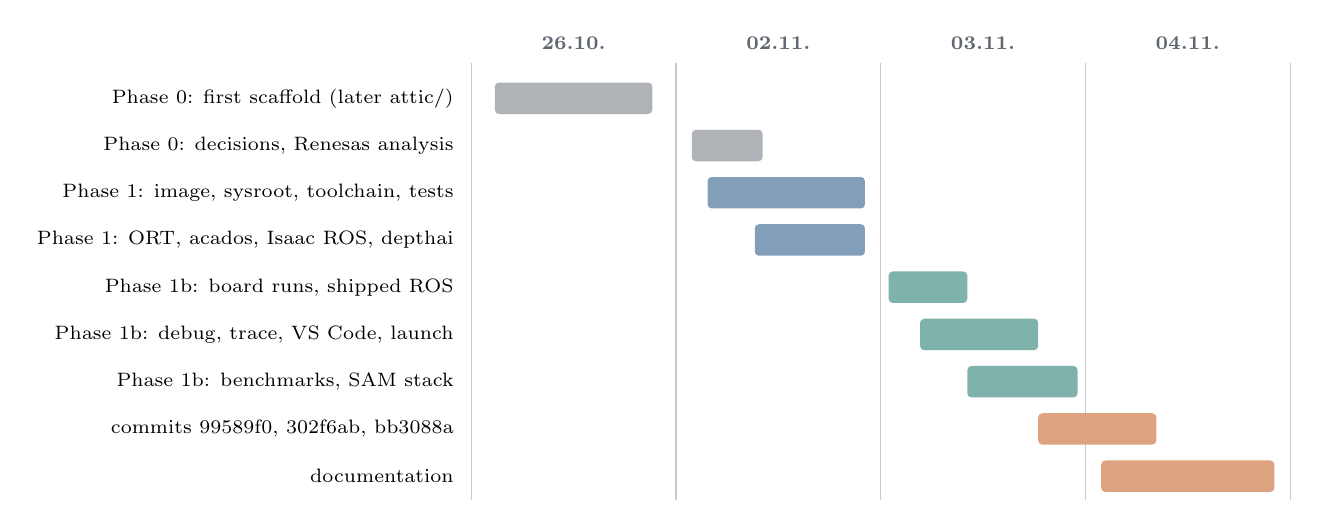
\begin{tikzpicture}[x=1cm,y=1cm]
  \foreach \x/\d in {1.0/26.10., 3.6/02.11., 6.2/03.11., 8.8/04.11.}{
    \node[font=\scriptsize\bfseries, text=jxbgray] at (\x,0.5) {\d};
    \draw[jxbgray!35] (\x-1.3,0.25) -- (\x-1.3,-5.3);
  }
  \draw[jxbgray!35] (10.1,0.25) -- (10.1,-5.3);
  \foreach \y/\t/\a/\b/\c in {
      -0.2/{Phase 0: first scaffold (later \code{attic/})}/0.0/2.0/jxbgray!50,
      -0.8/{Phase 0: decisions, Renesas analysis}/2.5/3.4/jxbgray!50,
      -1.4/{Phase 1: image, sysroot, toolchain, tests}/2.7/4.7/jxbblue!60,
      -2.0/{Phase 1: ORT, acados, Isaac ROS, depthai}/3.3/4.7/jxbblue!60,
      -2.6/{Phase 1b: board runs, shipped ROS}/5.0/6.0/jxbteal!60,
      -3.2/{Phase 1b: debug, trace, VS Code, launch}/5.4/6.9/jxbteal!60,
      -3.8/{Phase 1b: benchmarks, SAM stack}/6.0/7.4/jxbteal!60,
      -4.4/{commits \code{99589f0}, \code{302f6ab}, \code{bb3088a}}/6.9/8.4/jxborange!60,
      -5.0/{documentation}/7.7/9.9/jxborange!60}{
    \node[font=\scriptsize, anchor=east] at (-0.4,\y) {\t};
    \fill[\c, rounded corners=1.5pt] (\a,\y-0.2) rectangle (\b,\y+0.2);
  }
\end{tikzpicture}
\caption{Implementation timeline (days with activity; the columns are not to scale).}\label{fig:timeline}
\end{figure}

\subsection{Method}
\begin{itemize}
  \item \textbf{Evidence-driven engineering.} Every non-obvious observation was recorded as a numbered finding together
        with its consequence for the system before the next step; the findings log serves as design rationale and as
        regression list.
  \item \textbf{Probe-first verification.} Each capability has a minimal probe that exercises exactly one layer, so a
        failure points to its cause; only then is the full SAM workspace built.
  \item \textbf{Static checks of generated shell.} \jxb{} composes nested shell scripts (lock wrapper, container wrapper,
        environment, launch script). During development they were checked with \code{bash -n} through a dry-run harness
        that replaced the command runner and recursively checked every nested \code{bash -c} script.
  \item \textbf{Real hardware as the final test.} QEMU runs catch instruction-set and linkage errors early, but every
        feature was accepted only after it ran on the Nano.
  \item \textbf{Agent-assisted, parallel development.} The work was carried out with AI coding agents (Claude Code) under
        the direction of the project owner: a main development session, forked sessions for reviews and long
        measurement campaigns, and a separate hardware-in-the-loop session that shared the board. Coordination used
        explicit ownership of files and measurements and, on the board, the measurement lock, which the HIL session
        adopted. A forked review found the process-group issues of \cref{sec:launch} (\finding{58}).
\end{itemize}

\subsection{Incidents}
\begin{itemize}
  \item \textbf{Out-of-memory builds} (exit 137) on the 15\,GB host, resolved by bounding the parallelism (\finding{54}).
  \item \textbf{The board reset} of \finding{56}, which also interrupted other sessions on the shared board.
  \item \textbf{Lost work} when a session restored an earlier checkpoint and overwrote files; the changes were re-applied
        from the session transcript. Lesson: commit early on shared working trees.
\end{itemize}

% ======================================================================================================== 12
\section{Limitations and future work}\label{sec:limits}
Open issues of the current state:
\begin{itemize}
  \item \textbf{One board.} Only one Orin Nano was available. Several boards were tried as two inventory names for it
        (\finding{78}); parallel recordings on separate boards are untested. AGX Orin and Thor (GPU variant
        \code{openrm}) are prepared in the profile format but untested.
  \item \textbf{The RT kernel's memory-cgroup bug} (\finding{79}, \finding{85}) is NVIDIA's to fix. It reset the board
        three times in eight days, under load and without; \jxb{} notices a reset and \code{jxb board check} shows
        whether the last boot followed a crash.
  \item \textbf{Kernel traces of heavy loads} need large ring buffers, about 50\,MB per CPU for 30\,s of the full stack
        (\finding{80}); \jxb{} reports the loss and the size needed, but doesn't stream the trace.
  \item \textbf{The Basler Pylon SDK} needs its licence accepted; \code{pylon_camera_package} is the one SAM package not
        built.
\end{itemize}
Planned next steps (\code{PLAN.md}): ROS~2 tracing in container mode; an \code{orin-agent} daemon with a stable API (health, deploy,
run, logs, trace) as the common back end of \jxb{} and the later JetsonPlanner GUI, which needs a decision about
services on shared boards; and a provisioning bundle on top of stock JetPack (apt repository with cross-built packages,
container images, configuration) versioned together with the sysroot's package lock, which needs a board that may be
reflashed. Done since the first version of this document: multi-board commands and synchronized Perfetto timelines
(\cref{sec:fleet,sec:timeline}), CUDA kernel debugging (\cref{sec:debug}), GUI windows, CI, ros2\_control and Gazebo in
the Lyrical sysroots (\finding{74}), ROS~2 callback tracing (\cref{sec:rostrace}), the analyst's guide, and the Lyrical runtime fixes (\finding{68}, \finding{69}).

% ======================================================================================================== 13
\section{Conclusion}
\jxb{} shows that a correct cross-development environment for Jetson Orin can be \emph{constructed} rather than copied.
A private apt instance resolves the board's package closure from the board's own repositories; extraction plus a small,
explicit emulation of maintainer-script effects yields a sysroot that matches the board by construction; and a toolchain
whose defaults are pinned to the board compiles C++, CUDA and Python extensions without emulation. The same sysroot
doubles as the root file system of a GPU-enabled runtime container, which lets one stock board run three ROS
distributions natively or in a container. On top, a launch mode with process-group lifecycle management and an
observability pipeline with machine-readable summaries turn the board into a measurable system. Most of the effort went
into details that are invisible when building natively, such as symbolic-link semantics, \code{DT_NEEDED} records,
generated paths, undeclared dependencies and process lifecycles; documenting them, as this report and the findings log
do, is what makes the system maintainable.

% ======================================================================================================== appendix
\appendix
\section{Command reference}\label{app:commands}
\begin{longtable}{@{}>{\raggedright\arraybackslash}p{7.6cm}>{\raggedright\arraybackslash}p{8.3cm}@{}}
\toprule
Command & Purpose \\
\midrule
\endhead
\path{jxb image build | runtime} & build the xbuild image / the board runtime image of the profile \\
\path{jxb sysroot build [--add PKG ...] [--no-update]} & build the sysroot from the board's repositories \\
\path{jxb sysroot rosdeps -w WS} & workspace rosdeps and launch-file dependencies as package set \\
\path{jxb sysroot info} & metadata of the current sysroot \\
\path{jxb up [-w WS ...] [--recreate]}, \code{jxb down} & create / remove the dev container \\
\path{jxb shell}, \code{jxb exec -- CMD} & shell or command in the dev container \\
\path{jxb build [colcon args]} & \code{cross-colcon-build} in the current workspace \\
\path{jxb test [--board B]} & build and check the test suite, optionally run it on a board \\
\path{jxb board list | check B} & inventory; compare a board's package versions with \code{packages.lock} \\
\path{jxb deploy B [--ws WS] [--packages P ...] [--no-files]} & deploy a workspace \\
\path{jxb run B -- CMD}, \code{jxb ssh B} & command or shell on the board with the deployment's environment \\
\path{jxb gui B -- PROGRAM} & a board program as a window here (X11 over SSH) \\
\path{jxb launch B [--packages ...] [--monitor] [--bag [T ...]] [--with CMD] [--rates T ...] [--mem-guard MB] [--ros-trace] [--duration S] -- TARGET} & deploy and launch, optionally recorded \\
\path{jxb debug B --pkg P --exe E [--launch PKG FILE] [--server-only] [--cuda]} & remote debugging (\code{--cuda}: cuda-gdbserver and cuda-gdb) \\
\path{jxb gdb [--cuda] [-- ARGS]} & cross gdb (or cuda-gdb) for the profile \\
\path{jxb trace nsys | tegrastats | kernel | bench | ros B ...} & recordings on the board (\code{ros}: ROS~2 callbacks with LTTng) \\
\path{jxb trace report | plot | compare | perfetto | list | gui} & analysis on the host; \code{perfetto}: one timeline of recordings \\
\path{jxb vscode init -w WS [--board B ...] [--pkg P --exe E]} & VS Code workspace (several \code{--board}: debugging on all of them at once) \\
\bottomrule
\end{longtable}
\noindent Global options: \code{--profile NAME}, \code{--mode auto|native|container}, \code{--dry-run} (prints the
commands instead of running them). The board argument of \code{deploy}, \code{run}, \code{launch}, \code{test --board},
\code{board check} and the recordings also takes \code{B,B}, \code{@GROUP} or \code{all}: the command runs on those
boards at once, with a result table.

\section{Configuration reference}\label{app:config}
\begin{longtable}{@{}>{\raggedright\arraybackslash}p{6.4cm}>{\raggedright\arraybackslash}p{9.5cm}@{}}
\toprule
Key & Meaning \\
\midrule
\endhead
\multicolumn{2}{@{}l}{\textit{Profile} (\code{profiles/<name>.toml})} \\
\code{inherit} & parent profile; tables merge recursively \\
\code{[board]} \code{jetpack}, \code{l4t}, \code{soc}, \code{cpu_flags}, \code{cuda_arch}, \code{gpu_variant}, \code{ros_distro}, \code{ros_mode}, \code{qemu_cpu} & the board's software and hardware \\
\code{[image]} \code{tag}, \code{ubuntu}, \code{ros_distro}, \code{ros_apt_url}, \code{cuda_version}, \code{cuda_pkg_version} & build arguments of the xbuild image \\
\code{[sysroot]} \code{dir}, \code{codename}, \code{python}, \code{cuda_target}, \code{sources}, \code{preferences}, \code{package_sets}, \code{extras}, \code{rosdep_fallback_codename} & the sysroot recipe \\
\code{[keys]} & apt keyrings (paths or URLs) \\
\code{[extras.<name>]} & \code{tarball}, \code{debs} or \code{url}; \code{dest}, \code{optional}, \code{build} \\
\code{[container] board_paths} & board paths mapped into the dev container \\
\code{[deploy] runtime}, \code{container} & shipped runtime extras; forced container mode \\
\midrule
\multicolumn{2}{@{}l}{\textit{Boards} (\code{boards.toml}, local)} \\
\code{[defaults]}, \code{[boards.<name>]} & \code{host}, \code{user}, \code{ssh_port}, \code{deploy_dir}, \code{codename}, \code{gdb_port}, \code{nsys}, \code{trace_dir}, \code{measure_lock}, \code{trt_cache}, \code{cuda_gdbserver}, \code{groups} (for \code{@GROUP}), \code{ros_domain_id} \\
\midrule
\multicolumn{2}{@{}l}{\textit{Local defaults} (\code{jxb.toml}, local)} \\
\code{profile}, \code{mode}, \code{workspaces} & defaults for \code{--profile}, \code{--mode} and the dev container \\
\code{[sysroot] extra_sets} & additional package sets, e.g.\ \codeb{ws-{profile}-<ws>} \\
\code{[workspace.<dir>]} \code{files}, \code{env}, \code{container_env} & deployed source-tree files; board environment; extra variables in container mode \\
\bottomrule
\end{longtable}

\section{The \texorpdfstring{\codeb{summary.json}}{summary.json} schema}\label{app:summary}
\begin{longtable}{@{}l>{\raggedright\arraybackslash}p{2.6cm}>{\raggedright\arraybackslash}p{10.1cm}@{}}
\toprule
Key & Present for & Content \\
\midrule
\endhead
\code{trace}, \code{dir}, \code{meta} & all & name, directory, \code{meta.json} \\
\code{board_state} & all (since 2026-11-04) & \code{start}, \code{end}: \code{nvpmodel}; \codeb{cpu.<policy>} (\code{governor}, \code{min_mhz}, \code{max_mhz}, \code{cur_mhz}, \code{hw_min_mhz}, \code{hw_max_mhz}); \codeb{devfreq.<device>} (\code{governor}, \code{min_mhz}, \code{max_mhz}, \code{cur_mhz}; GPU, EMC = \code{bwmgr}, engines); \code{cpuidle} (\code{states}, \code{disabled}); \code{gpu_railgate}; \code{fan}; \code{temp_c}; \code{fixed} (clocks with minimum = maximum, disabled idle states); \code{changed} (settings that differ between start and end) \\
\code{ros} & \code{--ros-trace}, \code{trace ros} & \code{span_s}, \code{events}, \code{callbacks_run}, \code{nodes}; \code{callbacks[]} (\code{what}, \code{node}, \code{process}, \code{symbol}, \code{n}, \code{mean_ms}, \code{p50_ms}, \code{p99_ms}, \code{max_ms}, \code{total_ms}, \code{busy_pct}); \code{topics[]} (\code{publish_hz}, \code{takes}, \code{latency_p50_ms}, \code{latency_p99_ms}); \code{discarded_events} \\
\code{nsys} & nsys & \code{span_s}; \code{gpu} (\code{kernel_launches}, \code{kernel_time_ms}, \code{busy_ms}, \code{busy_pct}, \code{top_kernels}); \code{memcpy}; \code{cuda_api}; \code{nvtx}; \code{os_runtime}; \code{cpu_samples}; \code{processes} \\
\code{tegrastats} & monitored runs & \code{samples}, \code{interval_ms}, \code{duration_s}, \codeb{metrics.<key>.{mean,min,max}}, \code{energy_j}, \code{csv} \\
\code{processes} & \code{--monitor} & \code{session_cpu_pct}, \code{session_rss_mb}, \code{monitor_cpu_pct}; \code{session[]}, \code{top[]} with \code{cpu_share_pct}, \code{cpu_mean_pct}, \code{cpu_max_pct}, \code{rss_max_mb}, \code{series} \\
\code{launch} & launch & \code{processes}, \code{finished_cleanly}, \code{died}, \code{crashed}, \code{errors}, \code{warnings}, \code{first_errors} \\
\code{bag} & \code{--bag} & topics with type, message count and rate; CSV series of numeric topics \\
\code{kernel} & kernel & \code{span_s}, \code{events}, \code{ctxsw_per_s}, \code{cpu_busy_pct}, \code{top_tasks} (with \code{wakeup_us}), \code{top_processes}, \code{irqs} \\
\code{bench} & bench & per model: runs sorted by p50 with \code{p50_ms}, \code{p99_ms}, \code{fps}, \code{speedup_vs_ort_cuda} \\
\bottomrule
\end{longtable}

\section{FAQ and known issues}\label{app:faq}
\paragraph{Why not just build on the board?} It works for small packages, but the Orin Nano has 8\,GB of memory shared
between CPU and GPU and six cores; building there also requires \code{-dev} packages on a board that should stay stock.

\paragraph{Why not QEMU?} Emulated compilation is roughly an order of magnitude slower, and \code{nvcc} under emulation
was unreliable (P2). \jxb{} uses QEMU only for optional smoke tests.

\paragraph{Can I use my own CMake project without colcon?} Yes: in the dev container, run
\code{source /opt/jxb/toolchain/env.sh} and configure with \code{-DCMAKE_TOOLCHAIN_FILE=$JXB_TOOLCHAIN_FILE}.

\paragraph{\codeb{jxb board check} shows \codeb{DIFF}.} Patch-level differences within a release are ABI-compatible
(\finding{35}). Major differences mean that the board is not on the profile's JetPack release.

\paragraph{A node finds the wrong ONNX Runtime.} \jxb's GPU build comes first on \code{LD_LIBRARY_PATH} only in \jxb's
environment (\code{jxb run}, \code{jxb launch}, \code{jxb ssh}); a plain SSH shell sees the board's CPU-only
\code{/opt/onnxruntime}.

\paragraph{Known issues.} The RT kernel panics now and then in memory-cgroup accounting (\finding{79}, \finding{85}; it reset the board during \finding{56}), so ONNX Runtime's CUDA EP stays off in container mode; \code{pylon_camera_package} needs the Basler SDK; \code{micro_ros_agent} fails on
Kilted because its vendored Fast DDS references \code{tinyxml2::tinyxml2} (\finding{54}).

\section{Glossary}\label{app:glossary}
\begin{longtable}{@{}>{\raggedright\arraybackslash}p{3.2cm}>{\raggedright\arraybackslash}p{12.7cm}@{}}
\toprule
Term & Meaning \\
\midrule
\endhead
ABI & application binary interface: calling convention, data layout and symbol versions that binaries rely on \\
CDI & Container Device Interface, a specification of device nodes and mounts for containers \\
closure & the set of packages reachable through dependencies from the requested ones \\
EP & ONNX Runtime execution provider (CPU, CUDA, TensorRT) \\
fp16, INT8, Q/DQ & half precision; 8-bit integer; explicit quantize/dequantize nodes in an ONNX model \\
L4T & Linux for Tegra, NVIDIA's board support package (Jetson Linux) \\
merged \code{/usr} & layout in which \code{/bin}, \code{/lib} and \code{/sbin} are symbolic links into \code{/usr} \\
PREEMPT\_RT & the real-time preemption patch set of the Linux kernel \\
SBSA & Arm Server Base System Architecture; NVIDIA's unified Arm CUDA target layout \\
\code{SONAME} & the name a shared library declares for itself, recorded by the linker in \code{DT_NEEDED} \\
sysroot & a directory that compiler and linker treat as the target's root file system \\
underlay, overlay & an installed ROS environment; a workspace built on top of it \\
\bottomrule
\end{longtable}

% ======================================================================================================== references
\begin{thebibliography}{99}\small
\bibitem{renesas-devguide} Renesas Electronics. \emph{RZ/V2H RDK documentation: Development guide.}
  \url{https://renesas-rdk.github.io/rzv2h_rdk_documentation/latest/chapter-4/development_guide/development_guide.html}
\bibitem{renesas-setup} Renesas Electronics. \emph{RZ/V2H RDK documentation: Cross build setup.}
  \url{https://renesas-rdk.github.io/rzv2h_rdk_documentation/latest/chapter-4/development_guide/cross_build_setup.html}
\bibitem{renesas-vscode} Renesas Electronics. \emph{RZ/V2H RDK documentation: VS Code workspace.}
  \url{https://renesas-rdk.github.io/rzv2h_rdk_documentation/latest/chapter-4/development_guide/vs_code_ws.html}
\bibitem{renesas-faq} Renesas Electronics. \emph{RZ/V2H RDK documentation: Cross build FAQ.}
  \url{https://renesas-rdk.github.io/rzv2h_rdk_documentation/latest/chapter-4/development_guide/cross_build_faq.html}
\bibitem{renesas-toolchains} Renesas RDK. \emph{ubuntu\_xbuild\_toolchains.} \url{https://github.com/renesas-rdk/ubuntu_xbuild_toolchains}
\bibitem{nvidia-jetson} NVIDIA. \emph{Jetson Linux and JetPack documentation.} \url{https://docs.nvidia.com/jetson/}
\bibitem{nvcc} NVIDIA. \emph{CUDA Compiler Driver NVCC.} \url{https://docs.nvidia.com/cuda/cuda-compiler-driver-nvcc/}
\bibitem{nsys} NVIDIA. \emph{Nsight Systems User Guide.} \url{https://docs.nvidia.com/nsight-systems/UserGuide/}
\bibitem{cccl-8833} NVIDIA. \emph{CCCL issue 8833.} \url{https://github.com/NVIDIA/cccl/issues/8833}
\bibitem{cmake-toolchains} Kitware. \emph{cmake-toolchains(7).} \url{https://cmake.org/cmake/help/latest/manual/cmake-toolchains.7.html}
\bibitem{colcon} colcon contributors. \emph{colcon documentation.} \url{https://colcon.readthedocs.io/}
\bibitem{ros2-docs} Open Robotics. \emph{ROS~2 documentation.} \url{https://docs.ros.org/}
\bibitem{ftrace} The Linux kernel documentation. \emph{ftrace -- Function Tracer.} \url{https://www.kernel.org/doc/html/latest/trace/ftrace.html}
\bibitem{cdi} CNCF. \emph{Container Device Interface.} \url{https://github.com/cncf-tags/container-device-interface}
\bibitem{debian-policy} Debian. \emph{Debian Policy Manual.} \url{https://www.debian.org/doc/debian-policy/}
\bibitem{elf-gabi} \emph{System V Application Binary Interface (ELF).} \url{https://refspecs.linuxfoundation.org/elf/gabi4+/contents.html}
\end{thebibliography}

\end{document}
